% Chapter 6

\chapter{Experiments} % Write in your own chapter title
\label{Chapter6}
\lhead{Chapter \ref{Chapter6}. \emph{Experiments}} 

{\bf \small{
small  }}

\section{Introduction}



\section{Convex Multi-Task Learning with Kernel Methods}\label{subsec:convexmtlsvm_exp}
In this subsection we show the experiments used to test the convex \acrshort{mtl} formulation with kernel models, which have been presented in~\citep{RuizAD19} and~\citep{RuizAD21}. 
%
First, following the work in~\citep{RuizAD19}, experiments comparing convex and additive \acrshort{mtl} formulations in the L1-\acrshort{svm} are described. 
%
Then, the experiments of~\citep{RuizAD21} are exposed, where all convex \acrshort{mtl} models using L1, L2 and LS-\acrshort{svm}s as well as optimal convex combination of pre-trained models are compared over multiple real problems.

Before diving into the results, some technical details have to be explained. The convex \acrshort{mtl} formulation, as presented in Equation~\eqref{eq:svmmtl_primal_convex}, uses task-specific hyperparameters $\lambda_r$, as well as common and task-specific kernels, with their corresponding hyperparameters; however, the selection of many hyperparameters is always a challenge because of the curse of dimensionality. 
%
To select the hyperparameters $p_1, \ldots, p_L$ of a learning algorithm using CV the following problem is solved:
\begin{equation}
    \label{eq:hp-selection_general}
    p_1^*, \ldots, p_L^* = \argmin_{p_i \in \mathcal{S}_{p_i}, i=1, \ldots, L} \sum_{j=1}^{F} \rho(\mathcal{A}(p_1, \ldots, p_L; (X^j_\text{train}, y^j_\text{train})); (X^j_\text{val}, y^j_\text{val})) ,
\end{equation}
where $\rho$ is some measure; $\mathcal{A}$ is our choice of learning algorithm; $p_1, \ldots, p_L$ are the parameters on which $\mathcal{A}$ depends and $\mathcal{S}_{p_i}$ a feasible space for the parameter $p_i$; and $(X^j_\text{train}, y^j_\text{train}), (X^j_\text{val}, y^j_\text{val})$ are the training and validation sets, respectively. We are using $F$ folds, that is, for $j=1, \ldots, F$ we select different training and validation sets and we train our algorithm $\mathcal{A}$ on the training set $(X^j_\text{train}, y^j_\text{train})$; then we use $\rho$ to measure the wellness of our model on $(X^j_\text{val}, y^j_\text{val})$. 
%
Observe that our search space is the product space $\mathcal{S}_{p_1} \times \ldots \times \mathcal{S}_{p_L}$, so the difficulty of selecting an optimal combination of hyperparameters scales exponentially with the number of such parameters.

%
In a standard Gaussian kernel \acrshort{svm}, the definition of the classification problem depends on two hyperparameters: $C$ and $\gamma$.
For regression problems we also add a third parameter: $\epsilon$. 
That is, to select the hyperparameters of a standard \acrshort{svm} for a single task we have to solve the problem
\begin{equation}
    \nonumber
    C^*, \gamma^* (, \epsilon^*) = \argmin_{\substack{C \in \mathcal{S}_C ; \\ \substack{\gamma \in \mathcal{S}_\gamma} ; \\ \left(\substack{\epsilon \in \mathcal{S}_\epsilon} \right); }}
     \sum_{j=1}^{F} \rho(\mathcal{A}(C, \gamma (, \epsilon); (X^j_\text{train}, y^j_\text{train})); (X^j_\text{val}, y^j_\text{val})) ,
\end{equation}
which is typically feasible by using a grid search method in the space $\mathcal{S}_{C} \times \mathcal{S}_{\gamma} (\times \mathcal{S}_{\epsilon}) .$
%

However, using the convex \acrshort{mtl} formulation, 
%as shown in the \acrshort{mtl} kernel expression~\eqref{eq:conv_mtl_kernel_fun}, there are a common width $\gamma$ and task-specific widths $\gamma_1, \ldots, \gamma_\ntasks$.
we have the following hyperparameters: 
\begin{itemize}
    \item the regularization parameter $C$,
    \item the common kernel width $\gamma$ and task-specific ones $\gamma_1, \ldots, \gamma_\ntasks$,
    \item the convex combination parameters $\lambda_1, \ldots, \lambda_\ntasks$,
    \item and possibly the $\epsilon$ parameter.
\end{itemize}
That is, there are at least $2\ntasks + 2$ hyperparameters that have to be selected. Even with $\ntasks=2$, a search space of dimension $6$ is computationally unfeasible to cover with grid search.
% \begin{equation}
%     \nonumber
%     C^*, \gamma^*, \gamma_1^*, \ldots, \gamma_\ntasks^*, \lambda_1^*, \ldots, \lambda_\ntasks^*   (, \epsilon^*) = \argmin_{\substack{C \in \mathcal{S}_C ; \\ \substack{\gamma \in \mathcal{S}_\gamma} ; \\ \left(\substack{\epsilon \in \mathcal{S}_\epsilon} \right); }}
%      \sum_{j=1}^{F} \rho(\mathcal{A}(C, \gamma (, \epsilon); (X^j_\text{train}, y^j_\text{train})); (X^j_\text{val}, y^j_\text{val})) ,
% \end{equation}

To solve this difficulty and select the optimal parameters for the convex \acrshort{mtl} formulation we use the next strategy.
%
For the kernel widths, we proceed as follows: we first hyperparametrize the corresponding \acrshort{ctl} and \acrshort{itl} kernel models, which have a common and task-specific kernel widths, respectively. 
This step would give also optimal $C$ and $\epsilon$ values, but we discard them.
Observe that in the \acrshort{ctl} approach, where a single virtual task is solved, and in the \acrshort{itl} approach, where we solve the tasks independently, we have $2$ or $3$ hyperparameters. We solve the corresponding problems, which are represented in Equation~\eqref{eq:hp-selection_general}, using grid search, and we obtain optimal common $C^*, \gamma^*$ and task-specific ones $C_r^*, \gamma^*_r$ for $r=1, \ldots, \ntasks$ (also the respective $\epsilon^*$ values in the regression setting).
Then, we reutilize the optimal widths for these models, and fix them in the \acrshort{mtl} one.
%
Moreover, for the convex combination parameters we use a single $\lambda$ for all tasks, that is, $\lambda_1 = \ldots = \lambda_\ntasks = \lambda$.
%
With these considerations, the problem to select the remaining hyperparameters is 
\begin{equation}
    \nonumber
    C^*, \lambda^* (, \epsilon^*) = \argmin_{\substack{C \in \mathcal{S}_C ; \\ \substack{\lambda \in \mathcal{S}_\lambda} ; \\ \left(\substack{\epsilon \in \mathcal{S}_\epsilon} \right); }}
     \sum_{j=1}^{F} \rho(\mathcal{A}(C, \lambda, \gamma^*, \gamma_1^*, \ldots, \gamma_\ntasks^* (, \epsilon); (X^j_\text{train}, y^j_\text{train})); (X^j_\text{val}, y^j_\text{val})) ,
\end{equation}
where we have a maximum of $3$ hyperparameters.

%
In summary, these are the two adjustments that we make to carry out the experiments shown in this subsection.
The first adjustment concerning kernel widths does not change the model definition, but it assumes that kernel widths that are good for \acrshort{ctl} or \acrshort{itl} models are good for the \acrshort{mtl} one. 
Consider the Gaussian kernel
\begin{equation}
    \nonumber
    k(x, y) = \frac{1}{\sqrt{2\pi} \sigma}\exp{\left(-\frac{1}{2\sigma^2} (x-y)^2\right)},
\end{equation}
where $\sigma$ is the kernel width and it regulates ``how wide is the influence of each point'';
then, kernel widths are not that descriptive of the model but of the data used, which makes the reutilization of kernel widths a sensible decision.
The combined data from all tasks, which is used in \acrshort{ctl} approach, is well ``characterized'' by a width $\sigma^*$ so we expect that this width is also useful for the common part of the \acrshort{mtl} model. The same reasoning applies to task-specific data and \acrshort{itl} approach.
%
The second adjustment does change the models definition, using a single $\lambda$ that determines the specifity of all models. However, we expect that the possible difference in specifity among tasks can be corrected in the training process by selecting larger task-specific weights $v_r$ if necessary.

\paragraph*{Comparison of Convex and Additive Formulations\\}
% Figure Synthetic Problem HAIS2019
% \begin{figure}
%     \centering
%     \begin{subfigure}[b]{0.45\textwidth}
%         \centering
%         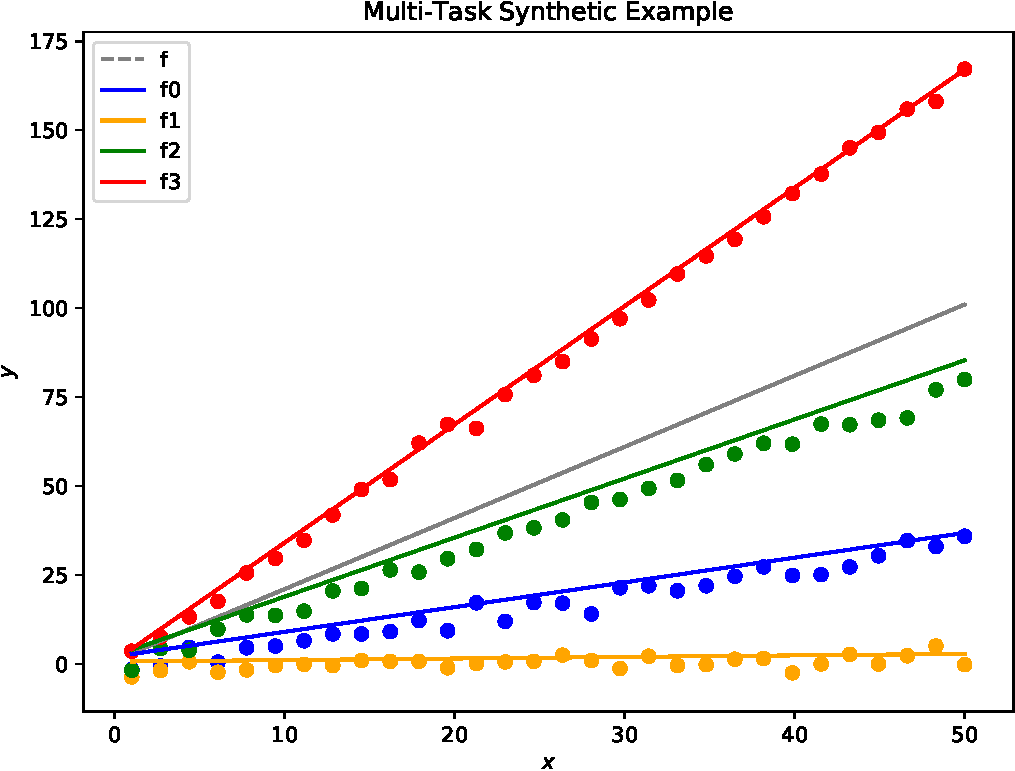
\includegraphics[width=\textwidth]{Chapter4/HAIS2019/synthetic_example-crop.pdf}
%     \end{subfigure}
%     \hfill
%     \begin{subfigure}[b]{0.45\textwidth}
%         \centering
%         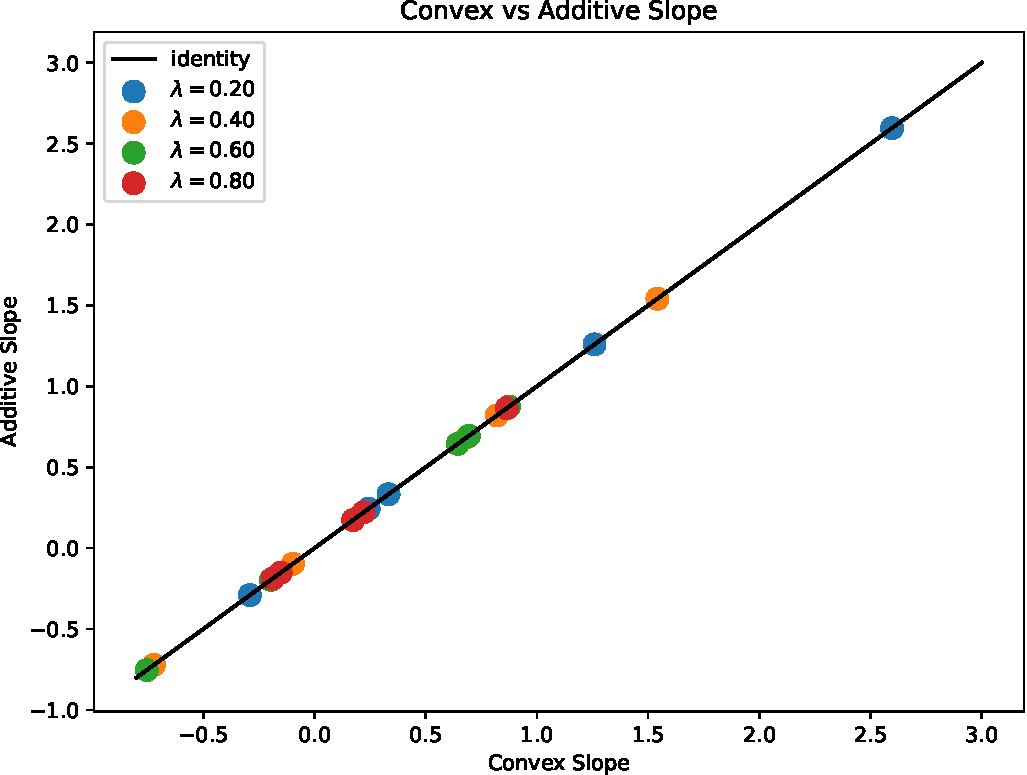
\includegraphics[width=\textwidth]{Chapter4/HAIS2019/synthetic_comparison-crop.pdf}
%     \end{subfigure}
%     \caption{Left: Synthetic example dataset, where the data of each task (corresponding to a different function $f_i$) are represented with a different color.
%         Right: Comparison of the weights obtained by the {convex} and {additive} approaches.}
%     \label{fig:lines_slopes}
% \end{figure}

\begin{figure}[t!]
    \centering
    \subfloat[][]{%    
    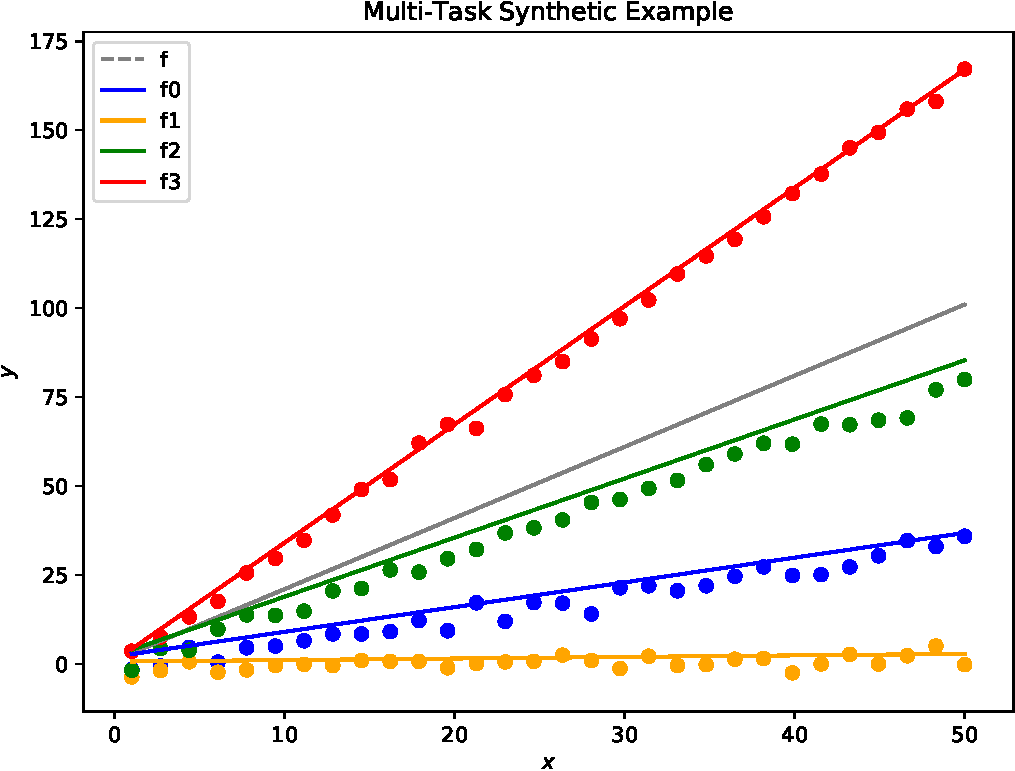
\includegraphics[width=0.45\textwidth]{Chapter4/HAIS2019/synthetic_example-crop.pdf}
    \label{fig:synthetic_example}}\quad%
    \subfloat[][]{%
    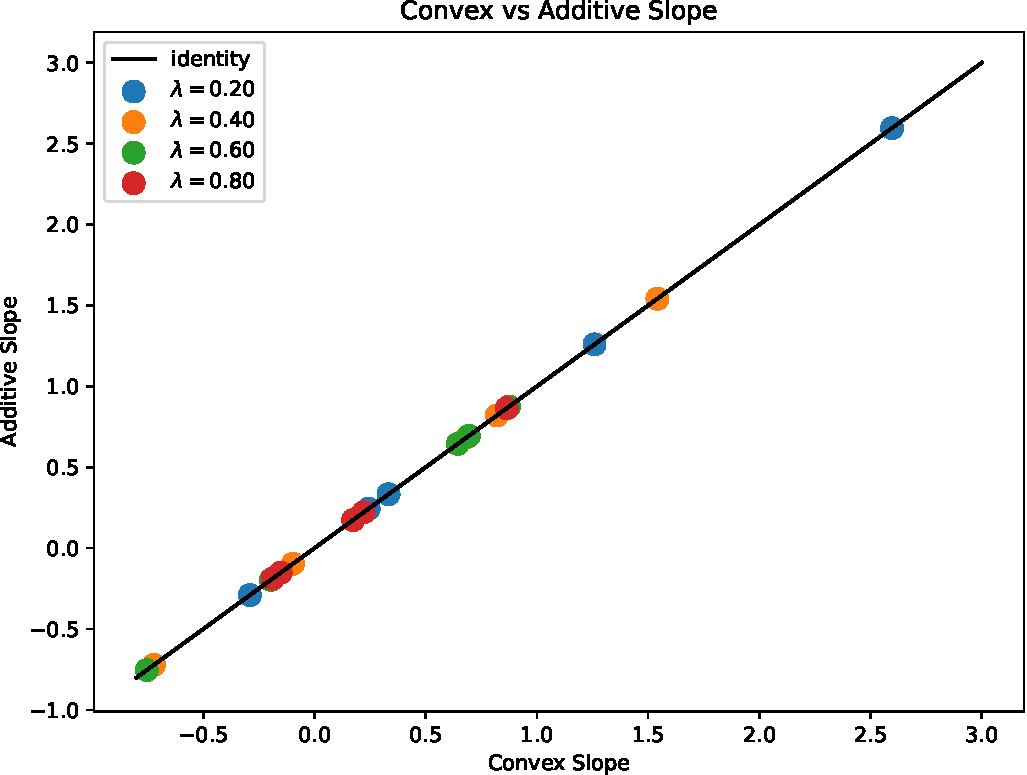
\includegraphics[width=0.45\textwidth]{Chapter4/HAIS2019/synthetic_comparison-crop.pdf}
    \label{fig:synthetic_comparison}}\\
    \caption{(\protect\subref{fig:synthetic_example}): Synthetic example dataset, where the data of each task (corresponding to a different function $f_i$) are represented with a different color.
    (\protect\subref{fig:synthetic_comparison}): Comparison of the weights obtained by the {convex} and {additive} approaches.}
    \label{fig:lines_slopes}
\end{figure}

% Figure Convex vs Additive HAIS2019
% \begin{figure}
%     \centering
%     \begin{subfigure}[b]{0.45\textwidth}
%         \centering
%         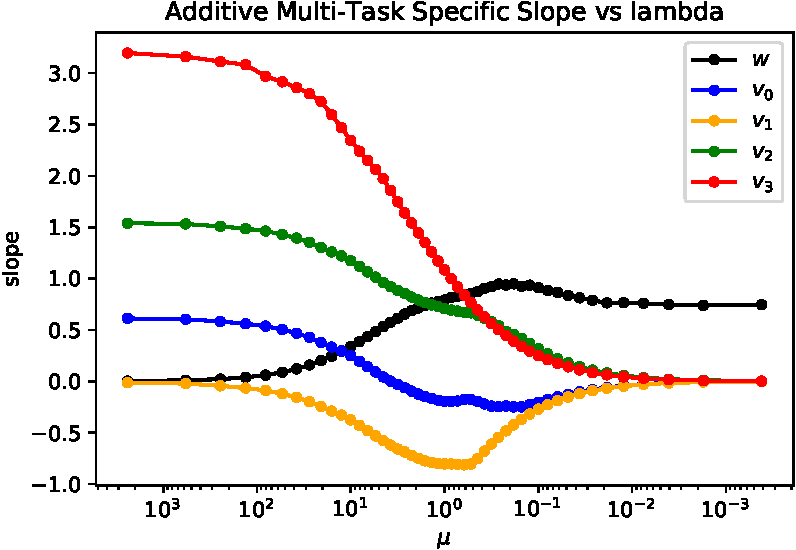
\includegraphics[width=\textwidth]{Chapter4/HAIS2019/synthetic_specWeights_add-crop.pdf}
%     \end{subfigure}
%     \hfill
%     \begin{subfigure}[b]{0.45\textwidth}
%         \centering
%         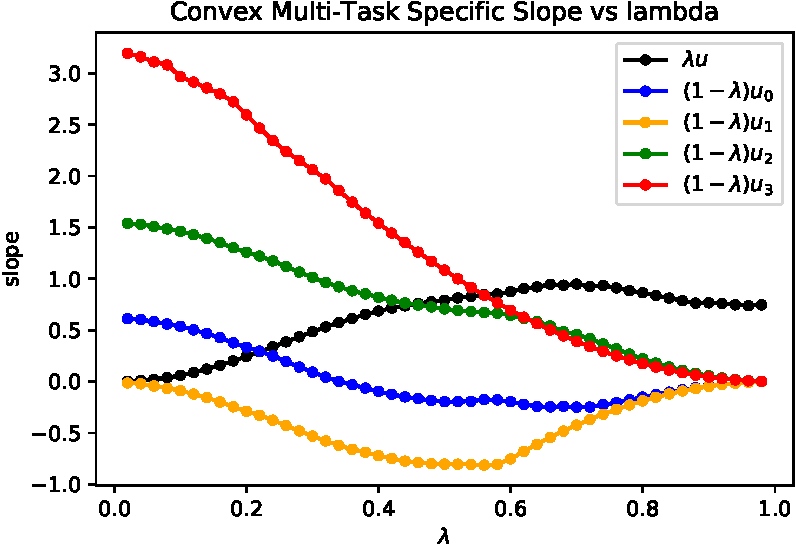
\includegraphics[width=\textwidth]{Chapter4/HAIS2019/synthetic_specWeights_conv-crop.pdf}
%     \end{subfigure}
%     \caption{{Convex} (right) and {additive} (left) MTLSVR slope estimates weights as a function of $\lambda$. We represent the common part of the models, $w$ for the {additive} and $\lambda u$ for the {convex}, as well as each task specific part $v_t$ and $(1 - \lambda) u_t$.}
%     \label{fig:synthetic_specWeights}
% \end{figure}

\begin{figure}[t!]
    \centering
    \subfloat[][]{%    
    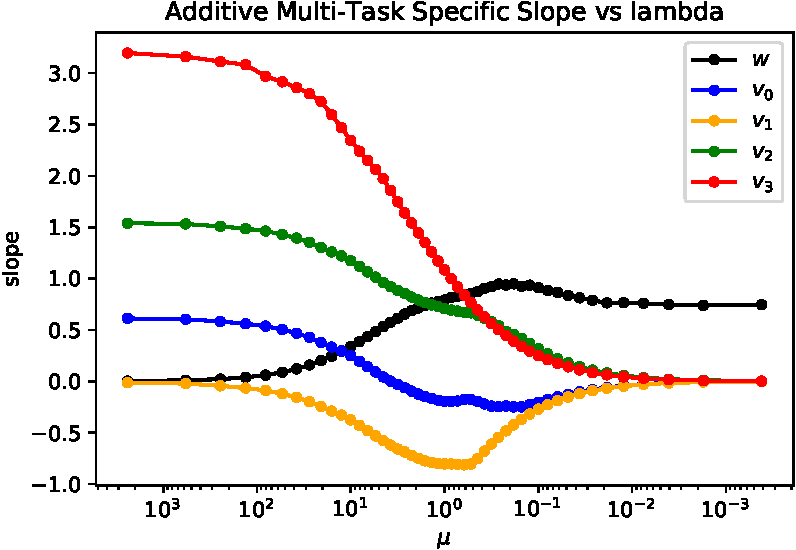
\includegraphics[width=0.45\textwidth]{Chapter4/HAIS2019/synthetic_specWeights_add-crop.pdf}
    \label{fig:additive_weights}}\quad%
    \subfloat[][]{%
    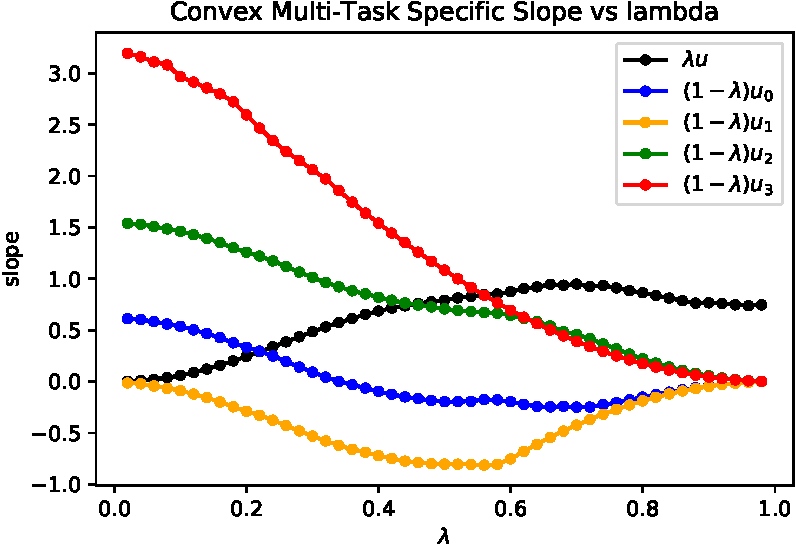
\includegraphics[width=0.45\textwidth]{Chapter4/HAIS2019/synthetic_specWeights_conv-crop.pdf}
    \label{fig:convex_weights}}\\
    \caption{{Convex} (\protect\subref{fig:convex_weights}) and {additive} (\protect\subref{fig:additive_weights}) MTLSVR slope estimates weights as a function of $\lambda$. We represent the common part of the models, $w$ for the {additive} and $\lambda u$ for the {convex}, as well as each task specific part $v_t$ and $(1 - \lambda) u_t$.}
    \label{fig:synthetic_specWeights}
\end{figure}



%The work shown in~\cite{RuizAD19} focuses on 

In~\citet{RuizAD19}, we illustrate the results of equivalence between the additive and convex formulations in an empirical way. To do this we generate a synthetic problem, shown in Figure~\ref{fig:synthetic_example}, as a four linear regression tasks problem. 
%
We use four different functions $f_0, f_1, f_2, f_3$ by considering a base function $f(x) = 2x - 1$ with slope $m=2$ and bias $n=1$, then we sample $z_m^r, z_n^r \sim \normal{0, 1}$ for each task $r=0, \ldots, 3$, and, create the $r$-th slope and bias by adding these Gaussian samples, i.e., $m_r = m + z_m^r$ and $n_r = n + z_n^r$. Also, we sample the noise level $\sigma_r$ for each task uniformly in $(0, 5)$. 
%
Then, the $r$-th task consists in estimating $m_r$ and $n_r$ from the data. To do this, for each task we uniformly sample $30$ points $x_i^r \in [1, 50)$, and the target values are defined as $y_i^r = f_r(x_i^r) + \epsilon^i_r$ where $\epsilon^i_r \sim \normal{0, \sigma_r}$.
%
Combining all tasks, there are $120$ data points, $30$ for each task, that we split randomly in a task-stratified way: two thirds, i.e. $80$ points are used for training, and the rest are used for testing purposes; in this division, the task size proportions are kept constant, that is $1/4$ for each task, in both the train and test sets. 
%
With this synthetic problem, we train four convex \acrshort{mtl} models corresponding to values of $\lambda \in \set{0.2, 0.4, 0.6, 0.8}$; and we also train the corresponding equivalent additive \acrshort{mtl} models, in which we set $\mu = (1 - \lambda)/\lambda^2$ and $C_\text{add} = (1 - \lambda)^2 C_\text{conv}$, as shown in Proposition~\ref{prop:add_conv_equiv}.
%
Our goal is to compare the influence of $\mu$ with that of $\lambda$ in the final models that are obtained. To do that, we need $C$ to be small enough so the regularization and, therefore, $\mu$ are relevant; the value $C_{\text{conv}} = 10^{-2}$ is found to be useful. We also consider linear kernels, so we can obtain the primal coefficients, that is, the slopes, and compare those obtained using the additive and convex formulations. In Figure~\ref{fig:synthetic_comparison}, we show the estimated slopes for each of the $\lambda$ values considered with a different color. In the $x$ axis we represent the slopes estimated using the convex approach and in the $y$ axis those estimated with the additive one. There are four dots of each color, corresponding to each of the tasks considered in our synthetic problem. We can observe that all dots lie in the diagonal line corresponding to the identity function, as we expected from the equivalence result from Proposition~\ref{prop:add_conv_equiv}.

%
To further compare the two formulations, we visualize how the change on the hyperparameters imposes a change on the final models. Using the already described synthetic problem of Figure~\ref{fig:synthetic_example}, left, we select values of $\lambda$ ranging from $0$ to $1$, and their corresponding values $\mu = (1-\lambda)^2 / \lambda^2$, and fit convex and additive \acrshort{mtl} linear \acrshort{svm}s using these values. In Figure~\ref{fig:synthetic_specWeights} we show the coefficients obtained for the common and task-specific parts with the additive formulation (left) and convex one (right).
%
We can observe how both graphics show a similar behaviour, with the common model starting in $0$ when $\mu$ is large or $\lambda=0$, and, as $\mu$ decreases and $\lambda$ grows, the task-specific parts go to zero and the common model reaches the optimal value for \acrshort{ctl}.
%

However, two facts are noticeable. The first one is the range of hyperparameters needed for each formulation; while the convex formulation always uses $[0, 1]$, with the additive formulation it seems that $(10^{-3}, 10^3)$ is useful in this problem, but we cannot extrapolate to other problems; the second one is the smoother transition of the convex formulation, where the changes are steadily made, while with the additive one the changes look more abrupt.



\paragraph*{Performance of Convex \acrshort{mtl} and Optimal Convex Combination.\\}

To test the performance of the convex \acrshort{mtl} formulation, in~\citet{RuizAD19} we also conduct experiments with real problems, which we later extend in~\citet{RuizAD21}. 
To test our proposal we apply it to three \acrshort{svm} variants: L1, L2 and LS-\acrshort{svm}. For each variant, we compare the \acrshort{ctl}, \acrshort{itl} with our convex \acrshort{mtl} formulation. To do this, we use fourteen different problems, six regression problems and eight classification ones.

% Models
\paragraph*{Models.}
Considering that {LX} can stand for {L1}, {L2} or {LS}, we use the following approaches:
\begin{itemize}
    \item {Common Task Learning LX-\acrshort{svm} (\fmod{\acrshort{ctl}-LX})}: A single LX-\acrshort{svm} fitted using data from all the tasks and does not use task information.
    \item {Independent Task Learning LX-\acrshort{svm} (\fmod{\acrshort{itl}-LX})}: Multiple task-specific LX-\acrshort{svm}s, each of which is fitted with the data from its own task.
    \item {Direct Convex Combination of LX-\acrshort{svm}s (\fmod{cvxCMB-LX})}: A combination of the best \fmod{\acrshort{ctl}-LX} and \fmod{\acrshort{itl}-LX} as described in Subsection~\ref{subsec:optimal_comb}.
    \item {Convex Multi-Task Learning LX-\acrshort{svm} (\fmod{cvxMTL-LX})}: The Convex \acrshort{mtl} formulations shown in Subsection~\ref{subsec:cvx_l1-svm} for the L1-\acrshort{svm} and in Subsection~\ref{subsec:cvx_l2ls-svm} for the L2- and LS-\acrshort{svm}.
\end{itemize}

% Problems
\paragraph*{Problems.}
To compare these approaches we will use several regression and classification problems. We use a total of six regression problems:
\begin{itemize}
    \item \fdata{majorca}: The goal is to predict the photovoltaic energy production in Mallorca. The tasks are defined as the energy prediction at each of the $14$ hours with sunlight (we remove the night hours).
    \item \fdata{tenerife}: The goal is to predict the photovoltaic energy production in Tenerife. The tasks are defined as the energy prediction at each of the $14$ hours with sunlight (we remove the night hours).
    \item \fdata{boston}\footnote{https://www.kaggle.com/datasets/schirmerchad/bostonhoustingmlnd}: This is the housing problem in Boston, where the goal is to predict house prices, and the tasks are defined as the predictions in different areas of the city. In Boston we have the houses that are next to the river and those that are not. 
    \item \fdata{california}\footnote{https://www.kaggle.com/datasets/camnugent/california-housing-prices}: This is the housing problem in California, where the goal is also to predict house prices. Here the tasks correspond to 4 different areas of California, according to their distance to the sea.
    \item \fdata{abalone}\footnote{https://archive.ics.uci.edu/ml/datasets/abalone}: The goal is to predict the number of rings of a specie of marine molluscs. The tasks are male, female or infant specimens.
    \item \fdata{crime}\footnote{https://archive.ics.uci.edu/ml/datasets/communities+and+crime}: The goal is to predict the number of crimes per \num{100000} habitants in the U.S., the tasks are the prediction of the crime rate in different states, and we consider nine states.
\end{itemize}
For the classification setting, we consider eight problems, six of which are generated by applying different task definitions to two different problems.
\begin{itemize}
    \item \fdata{landmine}\footnote{https://andreric.github.io/files/datasets/LandmineData\_19.mat}: This is a binary classification problem in which the goal is to detect landmines. Detection of different types of landmines define different tasks. 
    \item \fdata{binding}\footnote{https://github.com/pcpLiu/DeepSeqPan/tree/master/dataset}: This is a binary classification problem where the goal is to determine if a given molecule will bind with peptides. Different molecules define different tasks and the patterns are the characteristics of the peptides.
    \item \fdata{adult}\footnote{https://archive.ics.uci.edu/ml/datasets/adult}: The goal is to predict whether the yearly salary of a particular person is greater than 50K based on sociocultural data. We can define different tasks dividing the population by either gender or race, so we have the problems:
    \begin{itemize}
        \item \fdata{ad\_(G)}: dividing by gender. We consider $2$ tasks.
        \item \fdata{ad\_(R)}: dividing by race. We consider $5$ tasks.
        \item \fdata{ad\_(G, R)}: dividing by both gender and race, so we define a total of $10$ tasks.
    \end{itemize}
    \item \fdata{compas}\footnote{https://www.kaggle.com/datasets/danofer/compass}: The goal is to predict whether the COMPAS algorithm will assign "low" or "high" scores of recidivism to a particular subject. We can also divide the sample by either race or gender, so we obtain:
    \begin{itemize}
        \item \fdata{comp\_(G)}: dividing by gender. We consider $2$ tasks.
        \item \fdata{comp\_(R)}: dividing by race. We consider $4$ tasks
        \item \fdata{comp\_(G, R)}: dividing by both gender and race, so we define a total of $8$ tasks.
    \end{itemize}
\end{itemize}
% The characteristics of some of the problems considered are present in Table~\ref{tab:mtl_problems} but, considering the different task definitions for \fdata{compas} and \fdata{adult} 
We give in Table~\ref{tab:problems_hais19} a description of the characteristics of each problem.

% Table Problems HAIS19
\begin{table*}[t!]
    \caption{Sample sizes, dimensions and number of tasks of the datasets used.}
    \label{tab:problems_hais19}
    \centering
    \scalebox{.65}{
    \begin{tabular}{l*{7}{S[table-format=5]}}
    \toprule
    \fhead{Dataset} & \fhead{Size} & \fhead{No. feat.} & \fhead{No. tasks} & \fhead{Avg. task size} & \fhead{Min. t. s.} & \fhead{Max. t. s.}\\
    \midrule
    \fdata{majorca} & 15330 & 765 & 14 & 1095 & 1095 & 1095 \\ 
    \fdata{tenerife} & 15330 & 765 & 14 & 1095 & 1095 & 1095 \\
    \fdata{california} & 19269 & 9 & 5 & 3853 & 5 & 8468\\
    \fdata{boston} & 506 & 12 & 2 & 253 & 35 & 471 \\
    \fdata{abalone} & 4177 & 8 & 3 & 1392 & 1307 & 1527 \\
    \fdata{crime} & 1195 & 127 & 9 & 132 & 60  & 278 \\
    \fdata{binding} & 32302 & 184 & 47 & 687 & 59 & 3089 \\ 
    \fdata{landmine} & 14820 & 10 & 28 & 511 & 445 & 690 \\
    \fdata{adult\_(G)} & 48842 & 106 & 2 & 24421 & 16192 & 32650 \\
    \fdata{adult\_(R)} & 48842 & 103 & 5 & 9768 & 406 & 41762 \\
    \fdata{adult\_(G, R)} & 48842 & 101 & 10 & 4884 & 155 & 28735 \\
    \fdata{compas\_(G)} & 3987 & 11 & 2 & 1993 & 840 & 3147 \\
    \fdata{compas\_(R)} & 3987 & 9 & 4 & 997 & 255 & 1918 \\
    \fdata{compas\_(G, R)} & 3987 & 7 & 8 & 498 & 50 & 1525 \\
    \bottomrule
   \end{tabular}}
\end{table*}

% Experimental Procedure

% Table Hyperparameters HAIS19
\begin{table}[t]
    \caption{Hyperparameters, grids used to select them (when appropriate) and hyperparameter selection method for each model.}
    \label{tab:hyperpars_grid}
    \centering
    \scalebox{.65}{
     \begin{tabular}{*{9}{c}}
     \toprule
     \fhead{} & \fhead{Grid} & \fhead{\fmod{\acrshort{ctl}-L1,2}} & \fhead{\fmod{\acrshort{itl}-L1,2}} & \fhead{\fmod{cvxMTL-L1,2}}  & \fhead{\fmod{\acrshort{ctl}-LS}} & \fhead{\fmod{\acrshort{itl}-L,S}} & \fhead{\fmod{cvxMTL-LS}}   \\
     \midrule
      $C$ &  \scalebox{.9}{$\set{4^k: -2 \leq k \leq 6}$} & CV & CV & CV & CV & CV & CV  \\ 
      $\epsilon$ & \scalebox{.9}{$\set{\frac{\sigma}{4^k}: 1 \leq k \leq 6}$} & CV & CV & CV & - & - & - \\
      $\gamma_c$ & \scalebox{.9}{$\set{\frac{4^k}{d}: -2 \leq k \leq 3}$} & CV & - & \fmod{\acrshort{ctl}-L1,2} & CV & - & \fmod{\acrshort{ctl}-LS} \\
      $\gamma_s^r$ & \scalebox{.9}{$\set{\frac{4^k}{d}: -2 \leq k \leq 3}$} & - & CV & \fmod{\acrshort{itl}-L1,2} & - & CV & \fmod{\acrshort{itl}-LS}\\
      $\lambda$ & \scalebox{.9}{$\set{0.1 k : 0 \leq k \leq 10}$} & - & - & CV & - & - & CV \\
      \bottomrule
     \end{tabular}
     }
  \end{table}

\paragraph*{Experimental Procedure.}
To obtain the experimental results, we have to select the optimal hyperparameters for each model in a training-validation set and measure their performance on a test set. To do this, we follow the adjustments and experimental procedure described at the beginning of this subsection, reusing the kernel widths from \acrshort{ctl} and \acrshort{itl} approaches and limiting the convex \acrshort{mtl} formulation to a single convex combination hyperparameter $\lambda$.
%
In all models considered we use Gaussian kernels, so all features have been scaled to the $[0, 1]$ interval.
As previously explained, the hyperparameters for the \acrshort{ctl} and \acrshort{itl} approaches in the classification setting are $\set{C, \gamma}$ for all variants L1, L2 and LS-\acrshort{svm}.
In the regression setting we have $\set{C, \gamma, \epsilon}$ for the L1 and L2 variants, and $\set{C, \gamma}$ for the LS-\acrshort{svm}.
%
After selecting the optimal kernel widths in the \acrshort{ctl} approach $\sigma^*$, and the task-specific widths $\sigma_r^*$ in the \acrshort{itl} approach, we use these values to fix them in the convex \acrshort{mtl} formulation.
Then, the hyperparameters that we are considering for CV search in the convex \acrshort{mtl} approaches in the classification settings are $\set{C, \lambda}$ for all variants, while in the regression problems they are $\set{C, \lambda, \epsilon}$ for the L1 and L2 variants and $\set{C, \lambda}$ for the LS-\acrshort{svm}.
%
The optimal combination approaches do not have proper hyperparameters, since $\lambda$ is computed.
%
In all problems, the hyperparameters considered are selected with a grid search using a task-stratified $3$-fold CV. That is, given a training-validation set, we divide it in three different folds where the task proportions are kept constant, and we use two of these folds for training the model and evaluate its performance in the remaining one.
%
In the regression problems, we will measure the validation performance using the MAE, see Table~\ref{tab:error_models_reg_mae_mae}, and MSE, see Table~\ref{tab:error_models_reg_mse_mae}.  Observe that the objective function of L1-\acrshort{svm} based models is more aligned with minimizing the MAE, while those of L2 and LS-\acrshort{svm} based models are more related to minimizing the MSE.
In the classification problems, see Table~\ref{tab:error_models_class_f1}, we will consider the F1 score to deal with the class-imbalance ratio that we find, for example, in the \fdata{landmine} dataset where we have 200 negative examples for each 13 positive ones.
%
In Table~\ref{tab:hyperpars_grid} we show for each hyperparameter of the considered approaches whether they are selected using a CV procedure or recycling them from other approach, as well as the grids used for the CV search.

We have explained how we select the hyperparameters given a training-validation set, but it is necessary also to describe how we get the final test results that we present in the tables.
In every problem, except for \fdata{majorca} and \fdata{tenerife}, we will consider three external folds, each with the internal three folds for \acrshort{cv}. That is, the whole dataset of each problem is first divided in three task-stratified external folds: $F_1, F_
2, F_3$; then, two folds will form the training-validation set and the third one will be used as the test set. All folds have the same task proportions. There are three different combinations to do this division: $\set{F_1, F_2; F_3}, \set{F_1, F_3; F_2}$ and $\set{F_2, F_3; F_1}$, where the first two folds form the train-validation set and the other one is the test set.
%
In each train-validation set we follow the procedure described above to select the optimal hyperparameters, and the performance model with the optimal hyperparameters will be tested in the remaining fold, i.e., the test set.
%

The problems of \fdata{majorca} and \fdata{tenerife} have a temporal dependency, so it is not sensible to use training data from a time that is ahead of that of the test or validation data. Therefore, we use data from years 2013, 2014 and 2015, each corresponding to train, validation and test sets, respectively.
%
We consider different metrics to measure the test performance. Therefore, in every problem, except \fdata{majorca} and \fdata{tenerife}, for each metric we obtain three different scores, each corresponding to a different test set, so we will show the mean and standard deviation of such scores. In \fdata{majorca} and \fdata{tenerife} we obtain a single test score corresponding to data from the year 2015.
% 
For the regression problems, in Tables~\ref{tab:error_models_reg_mae_mae} and~\ref{tab:error_models_reg_mse_mae}, we show both the MAE and R2 score, closely related to MSE, obtained in the test set, and for classification, in Table~\ref{tab:error_models_class_f1}, we show the F1 and the accuracy scores.
%




% Results


  \begin{table*}[t]
    \captionsetup{font=scriptsize}
    \caption{Test \acrshort{mae} (top) and R2 score (bottom) and Wilcoxon-based ranking. Here, the optimal hyperparameters have been selected using the \acrshort{mae}. The best models are shown in bold.}
    \label{tab:error_models_reg_mae_mae}
    \centering
    \scalebox{.65}{
    \begin{tabular}{l*{2}{c@{ }l}*{4}{r@{$\pm$}l@{ }l } }
    \toprule
    & \fheadmulti{2}{\fdata{maj.}} & \fheadmulti{2}{\fdata{ten.}} & \fheadmulti{3}{\fdata{boston}} & \fheadmulti{3}{\fdata{california}} &  \fheadmulti{3}{\fdata{abalone}} & \fheadmulti{3}{\fdata{crime}}\\
    \midrule
    & \fheadmulti{16}{MAE} \\
    \midrule
    \fmod{\acrshort{itl}-L1}            &  {5.087} &   (6) &  {5.743} &   (3) &  {2.341} & {0.229} &   \fmaxn{(1)} &  {36883.582} & {418.435} &   (2) &  {1.481} & {0.051} &   (3) &  {0.078} & {0.001} &   (2) \\
    \fmod{\acrshort{ctl}-L1}            &  {5.175} &   (7) &  {5.891} &   (5) &  \fmaxn{2.192} & \fmaxn{0.244} &   \fmaxn{(1)} &  {41754.337} & {270.908} &   (6) &  {1.482} & {0.050} &   (3) &  {0.078} & {0.001} &   (2) \\
    \fmod{cvxCMB-L1} &  \fmaxn{5.047} &   (5) &  \fmaxn{5.340} &  \fmaxn{(1)} &  {2.239} & {0.255} &   \fmaxn{(1)} &  {36880.238} & {420.417} &   \fmaxn{(1)} &  {1.470} & {0.052} &   (2) &  {0.077} & {0.002} &   (2) \\
    \fmod{cvxMTL-L1}     &  {5.050} &   (5) &  {5.535} &   (2) &  {2.206} & {0.292} &   \fmaxn{(1)} &  \fmaxn{36711.383} & \fmaxn{343.333} &  \fmaxn{(1)} &  \fmaxn{1.454} & \fmaxn{0.048} &  \fmaxn{(1)} &  \fmaxn{0.074} & \fmaxn{0.002} &  \fmaxn{(1)} \\
    \midrule
    \fmod{\acrshort{itl}-L2}            &  {4.952} &   (3) &  \fmaxn{5.629} &   (3) &  {2.356} & {0.300} &   \fmaxn{(1)} &  {37374.618} & {433.511} &   (5) &  {1.498} & {0.054} &   (4) &  {0.079} & {0.002} &   (2) \\
    \fmod{\acrshort{ctl}-L2}            &  {5.193} &   (7) &  {6.107} &   (8) &  \fmaxn{2.083} & \fmaxn{0.136} &   \fmaxn{(1)} &  {42335.612} & {163.773} &   (8) &  {1.503} & {0.047} &   (5) &  {0.080} & {0.002} &   (2) \\
    \fmod{cvxCMB-L2} &  {4.869} &   (3) &  {5.963} &   (6) &  {2.089} & {0.128} &   \fmaxn{(1)} &  {37374.618} & {433.511} &   (4) &  {1.494} & {0.050} &   (4) &  {0.077} & {0.003} &   (2) \\
    \fmod{cvxMTL-L2}     &  \fmaxn{4.854} &   (2) &  {5.784} &   (4) &  {2.089} & {0.134} &   \fmaxn{(1)} &  \fmaxn{37202.603} & \fmaxn{419.166} &   (3) &  \fmaxn{1.482} & \fmaxn{0.049} &   (3) &  \fmaxn{0.077} & \fmaxn{0.002} &   (2) \\
    \midrule
    \fmod{\acrshort{itl}-LS}            &  {4.937} &   (3) &  {5.649} &   (3) &  {2.204} & {0.116} &   \fmaxn{(1)} &  {37348.347} & {441.240} &   (4) &  {1.496} & {0.051} &   (4) &  {0.079} & {0.002} &   (2) \\
    \fmod{\acrshort{ctl}-LS}            &  {5.193} &   (7) &  {6.005} &   (7) &  \fmaxn{2.072} & \fmaxn{0.143} &  \fmaxn{(1)} &  {42259.492} & {146.825} &   (7) &  {1.502} & {0.052} &   (5) &  {0.079} & {0.002} &   (2) \\
    \fmod{cvxCMB-LS} &  {4.977} &   (4) &  \fmaxn{5.593} &   (3) &  {2.081} & {0.146} &   \fmaxn{(1)} &  {37339.179} & {430.288} &   (4) &  {1.486} & {0.049} &   (4) &  {0.079} & {0.002} &   (2) \\
    \fmod{cvxMTL-LS}     &  \fmaxn{4.824} &  \fmaxn{(1)} &  {5.754} &   (4) &  {2.077} & {0.152} &   \fmaxn{(1)} &  \fmaxn{37231.043} & \fmaxn{420.992} &   (4) &  \fmaxn{1.478} & \fmaxn{0.050} &   (3) &  \fmaxn{0.076} & \fmaxn{0.002} &   (2) \\
    \midrule
    & \fheadmulti{16}{R2} \\
    \midrule
    \fmod{\acrshort{itl}-L1}            &  {0.845} &   (6) &  {0.901} &   (7) &  {0.821} & {0.041} &   (2) &  {0.699} & {0.009} &   (7) &  {0.543} & {0.022} &   (8) &  {0.732} & {0.021} &   (3) \\
    \fmod{\acrshort{ctl}-L1}            &  {0.837} &   (9) &  {0.901} &   (6) &  {0.854} & {0.036} &   \fmaxn{(1)} &  {0.639} & {0.006} &  (10) &  {0.559} & {0.014} &   (6) &  {0.740} & {0.027} &   (3) \\
    \fmod{cvxCMB-L1} &  {0.844} &   (6) &  {0.905} &   (4) &  {0.845} & {0.053} &   \fmaxn{(1)} &  {0.699} & {0.009} &   (6) &  {0.555} & {0.018} &   (7) &  {0.741} & {0.029} &   (3) \\
    \fmod{cvxMTL-L1}     &  \fmaxn{0.846} &   (4) &  \fmaxn{0.908} &   (2) &  \fmaxn{0.858} & \fmaxn{0.057} &   \fmaxn{(1)} &  \fmaxn{0.703} & \fmaxn{0.007} &   (6) &  \fmaxn{0.568} & \fmaxn{0.012} &   (5) &  \fmaxn{0.760} & \fmaxn{0.024} &   (2) \\
    \midrule
    \fmod{\acrshort{itl}-L2}            &  {0.846} &   (5) &  {0.906} &   (3) &  {0.836} & {0.045} &   (2) &  {0.707} & {0.009} &   (5) &  {0.565} & {0.025} &   (6) &  {0.743} & {0.017} &   (3) \\
    \fmod{\acrshort{ctl}-L2}            &  {0.840} &   (8) &  {0.901} &   (8) &  \fmaxn{0.889} & \fmaxn{0.017} &   \fmaxn{(1)} &  {0.645} & {0.005} &   (9) &  {0.574} & {0.013} &   (4) &  {0.744} & {0.028} &   (3) \\
    \fmod{cvxCMB-L2} &  {0.850} &   (3) &  {0.900} &   (9) &  {0.885} & {0.013} &   \fmaxn{(1)} &  {0.707} & {0.009} &   (4) &  {0.571} & {0.018} &   (4) &  {0.755} & {0.024} &   (3) \\
    \fmod{cvxMTL-L2}     &  \fmaxn{0.863} &   (2) &  \fmaxn{0.908} &   \fmaxn{(1)} &  {0.888} & {0.015} &   \fmaxn{(1)} &  \fmaxn{0.709} & \fmaxn{0.008} &  \fmaxn{(1)} &  \fmaxn{0.580} & \fmaxn{0.014} &   (3) &  \fmaxn{0.762} & \fmaxn{0.028} &   \fmaxn{(1)} \\
    \midrule
    \fmod{\acrshort{itl}-LS}            &  {0.849} &   (3) &  {0.907} &   (3) &  {0.856} & {0.008} &   \fmaxn{(1)} &  {0.707} & {0.009} &   (3) &  {0.573} & {0.015} &   (4) &  {0.743} & {0.022} &   (3) \\
    \fmod{\acrshort{ctl}-LS}            &  {0.838} &   (9) &  {0.904} &   (5) &  \fmaxn{0.894} & \fmaxn{0.015} &  \fmaxn{(1)} &  {0.646} & {0.005} &   (8) &  {0.576} & {0.016} &   (4) &  {0.746} & {0.032} &   (3) \\
    \fmod{cvxCMB-LS} &  {0.843} &   (7) &  {0.907} &   (2) &  {0.886} & {0.024} &   \fmaxn{(1)} &  {0.707} & {0.009} &   (2) &  {0.581} & {0.012} &   (2) &  {0.746} & {0.021} &   (3) \\
    \fmod{cvxMTL-LS}     &  \fmaxn{0.863} &  \fmaxn{(1)} &  \fmaxn{0.910} &  \fmaxn{(1)} &  {0.890} & {0.016} &   \fmaxn{(1)} &  \fmaxn{0.709} & \fmaxn{0.008} &   (2) &  \fmaxn{0.581} & \fmaxn{0.015} &  \fmaxn{(1)} &  \fmaxn{0.763} & \fmaxn{0.028} &  \fmaxn{(1)} \\
    \bottomrule
    \end{tabular}}
  \end{table*}





  \begin{table*}[t]
    \captionsetup{font=scriptsize}
    \caption{Test \acrshort{mae} (top) and R2 score (bottom) and Wilcoxon-based ranking. Here, the optimal hyperparameters have been selected using the \acrshort{mse}. The best models are shown in bold.}
      \label{tab:error_models_reg_mse_mae}
      \centering
      \scalebox{.65
      }{
          \begin{tabular}{l*{2}{c@{ }l}*{4}{r@{$\pm$}l@{ }l } }
              \toprule
              & \fheadmulti{2}{\fdata{maj.}} & \fheadmulti{2}{\fdata{ten.}} & \fheadmulti{3}{\fdata{boston}} & \fheadmulti{3}{\fdata{california}} &  \fheadmulti{3}{\fdata{abalone}} & \fheadmulti{3}{\fdata{crime}}\\
      \midrule
      & \fheadmulti{16}{MAE} \\
      \midrule
      \fmod{\acrshort{itl}-L1}            &  {5.087} &   (7) &  {5.743} &   (3) &  {2.437} & {0.281} &   (3) &  {36941.516} & {450.767} &   (1) &  {1.480} & {0.058} &   (3) &  {0.079} & {0.002} &   (3) \\
      \fmod{\acrshort{ctl}-L1}            &  {5.175} &   (8) &  {5.891} &   (7) &  {2.315} & {0.192} &   (2) &  {41857.602} & {235.021} &   (6) &  {1.479} & {0.047} &   (3) &  {0.078} & {0.000} &   (2) \\
      \fmod{cvxCMB-L1} &  \fmaxn{4.920} &   (4) &  {5.743} &   (4) &  {2.315} & {0.192} &   (3) &  \fmaxn{36941.476} & \fmaxn{450.711} &  \fmaxn{(1)} &  {1.471} & {0.057} &   (2) &  {0.079} & {0.002} &   (2) \\
      \fmod{cvxMTL-L1}     &  {5.050} &   (6) &  \fmaxn{5.535} &  \fmaxn{(1)} &  \fmaxn{2.244} & \fmaxn{0.150} &   (1) &  {36999.003} & {360.445} &   (2) &  \fmaxn{1.455} & \fmaxn{0.046} &  \fmaxn{(1)} &  \fmaxn{0.074} & \fmaxn{0.001} &  \fmaxn{(1)} \\
      \midrule
      \fmod{\acrshort{itl}-L2}            &  {4.924} &   (5) &  {5.752} &   (5) &  {2.437} & {0.324} &   (3) &  {37407.929} & {461.878} &   (5) &  {1.497} & {0.050} &   (5) &  {0.079} & {0.002} &   (2) \\
      \fmod{\acrshort{ctl}-L2}            &  {5.193} &   (8) &  {6.107} &   (9) &  {2.096} & {0.112} &   (1) &  {42335.612} & {163.773} &   (7) &  {1.504} & {0.048} &   (6) &  {0.079} & {0.002} &   (2) \\
      \fmod{cvxCMB-L2} &  \fmaxn{4.813} &  \fmaxn{(1)} &  \fmaxn{5.623} &   (3) &  {2.116} & {0.131} &   (1) &  {37398.940} & {449.498} &   (5) &  {1.495} & {0.051} &   (5) &  {0.078} & {0.003} &   (2) \\
      \fmod{cvxMTL-L2}     &  {4.854} &   (4) &  {5.784} &   (6) &  \fmaxn{2.082} & \fmaxn{0.130} &   (1) &  \fmaxn{37356.599} & \fmaxn{390.629} &   (4) &  \fmaxn{1.481} & \fmaxn{0.041} &   (4) &  \fmaxn{0.076} & \fmaxn{0.000} &   (2) \\
      \midrule
      \fmod{\acrshort{itl}-LS}            &  {4.937} &   (5) &  {5.649} &   (3) &  {2.326} & {0.231} &   (3) &  {37385.244} & {403.331} &   (4) &  {1.495} & {0.045} &   (5) &  {0.079} & {0.002} &   (2) \\
      \fmod{\acrshort{ctl}-LS}            &  {5.193} &   (8) &  {6.005} &   (8) &  \fmaxn{2.072} & \fmaxn{0.143} &  \fmaxn{(1)} &  {42339.063} & {156.624} &   (7) &  {1.504} & {0.043} &   (6) &  {0.078} & {0.002} &   (2) \\
      \fmod{cvxCMB-LS} &  \fmaxn{4.820} &   (2) &  {5.578} &   (2) &  {2.136} & {0.106} &   (1) &  {37377.005} & {391.694} &   (4) &  {1.491} & {0.048} &   (5) &  {0.078} & {0.002} &   (2) \\
      \fmod{cvxMTL-LS}     &  {4.824} &   (3) &  \fmaxn{5.754} &   (6) &  {2.090} & {0.090} &   (1) &  \fmaxn{37232.918} & \fmaxn{397.866} &   (3) &  \fmaxn{1.478} & \fmaxn{0.042} &   (3) &  \fmaxn{0.076} & \fmaxn{0.000} &   (2) \\
      \midrule
      & \fheadmulti{16}{R2} \\
      \midrule
      \fmod{\acrshort{itl}-L1}            &  {0.845} &   (6) &  {0.901} &   (9) &  {0.800} & {0.050} &   (3) &  {0.703} & {0.009} &   (8) &  {0.534} & {0.053} &  (10) &  {0.732} & {0.017} &   (4) \\
      \fmod{\acrshort{ctl}-L1}            &  {0.837} &   (7) &  {0.901} &   (8) &  {0.860} & {0.026} &   (2) &  {0.642} & {0.006} &  (10) &  {0.564} & {0.011} &   (8) &  {0.748} & {0.017} &   (3) \\
      \fmod{cvxCMB-L1} &  \fmaxn{0.852} &   (4) &  {0.901} &  (10) &  {0.860} & {0.026} &   (3) &  {0.703} & {0.009} &   (7) &  {0.550} & {0.036} &   (9) &  {0.733} & {0.018} &   (3) \\
      \fmod{cvxMTL-L1}     &  {0.846} &   (5) &  \fmaxn{0.908} &   (5) &  \fmaxn{0.871} & \fmaxn{0.019} &   (1) &  \fmaxn{0.705} & \fmaxn{0.008} &   (6) &  \fmaxn{0.573} & \fmaxn{0.011} &   (7) &  \fmaxn{0.764} & \fmaxn{0.019} &   (1) \\
      \midrule
      \fmod{\acrshort{itl}-L2}            &  {0.850} &   (4) &  {0.906} &   (6) &  {0.819} & {0.053} &   (3) &  {0.707} & {0.009} &   (4) &  {0.573} & {0.020} &   (6) &  {0.744} & {0.018} &   (3) \\
      \fmod{\acrshort{ctl}-L2}            &  {0.840} &   (6) &  {0.901} &  (11) &  {0.886} & {0.014} &   (1) &  {0.645} & {0.005} &   (9) &  {0.574} & {0.013} &   (6) &  {0.747} & {0.025} &   (3) \\
      \fmod{cvxCMB-L2} &  {0.857} &   (3) &  \fmaxn{0.910} &  \fmaxn{(1)} &  {0.883} & {0.016} &   (1) &  {0.707} & {0.009} &   (2) &  {0.574} & {0.021} &   (5) &  {0.751} & {0.029} &   (3) \\
      \fmod{cvxMTL-L2}     &  \fmaxn{0.863} &   (2) &  {0.908} &   (4) &  \fmaxn{0.887} & \fmaxn{0.015} &   (1) &  \fmaxn{0.708} & \fmaxn{0.007} &   (2) &  \fmaxn{0.581} & \fmaxn{0.011} &   (2) &  \fmaxn{0.768} & \fmaxn{0.020} &  \fmaxn{(1)} \\
      \midrule
      \fmod{\acrshort{itl}-LS}            &  {0.849} &   (4) &  {0.907} &   (5) &  {0.841} & {0.028} &   (3) &  {0.707} & {0.009} &   (5) &  {0.577} & {0.012} &   (4) &  {0.743} & {0.021} &   (3) \\
      \fmod{\acrshort{ctl}-LS}            &  {0.838} &   (7) &  {0.904} &   (7) &  \fmaxn{0.894} & \fmaxn{0.015} &  \fmaxn{(1)} &  {0.645} & {0.005} &   (9) &  {0.575} & {0.012} &   (4) &  {0.754} & {0.022} &   (3) \\
      \fmod{cvxCMB-LS} &  {0.856} &   (3) &  {0.909} &   (3) &  {0.877} & {0.009} &   (1) &  {0.707} & {0.009} &   (3) &  {0.580} & {0.013} &   (3) &  {0.750} & {0.024} &   (3) \\
      \fmod{cvxMTL-LS}     &  \fmaxn{0.863} &  \fmaxn{(1)} &  \fmaxn{0.910} &   (2) &  {0.890} & {0.014} &   (1) &  \fmaxn{0.710} & \fmaxn{0.008} &  \fmaxn{(1)} &  \fmaxn{0.582} & \fmaxn{0.011} &  \fmaxn{(1)} &  \fmaxn{0.763} & \fmaxn{0.019} &   (2) \\
      \bottomrule
      \end{tabular}}
    \end{table*}
  



\begin{table*}[t]
    \captionsetup{font=scriptsize}
    \caption{Test F1 (top) and accuracy (bottom) scores, global and block-wise Wilcoxon-based rankings for classification problems. The best models in each block are shown in bold.}
    \label{tab:error_models_class_f1}
    \centering
    \scalebox{.65}{
      \begin{tabular}{ l*{8}{c} c c c}
        \toprule
        & \fhead{\fdata{comp\_(G)}} & \fhead{\fdata{comp\_(R)}} & \fhead{\fdata{comp\_(G,R)}} & \fhead{\fdata{ad\_(G)}} & \fhead{\fdata{ad\_(R)}} & \fhead{\fdata{ad\_(G,R)}} & \fhead{\fdata{landmine}} & \fhead{\fdata{binding}} & \fhead{mean} & \fhead{rank} & \fhead{Wil.}\\
        \midrule
        & \fheadmulti{8}{F1}  \\
        \midrule
        \fmod{\acrshort{itl}-L1}    &          0.625 &           \fmaxn{0.639} &                  0.630 &         \fmaxn{0.659} &          0.653 &                 0.657 &    0.231 &   0.867 & 0.620 &     10 & 1 \\
        \fmod{\acrshort{ctl}-L1}    &          0.623 &           0.638 &                  0.638 &         0.657 &          0.650 &                 0.653 &    0.255 &   0.901 & 0.627 &      7 & 1 \\
        \fmod{cvxCMB-L1} &          0.616 &           0.638 &                  0.638 &         0.658 &          0.650 &                 0.653 &    \fmaxn{0.270} &   0.901 & \fmaxn{0.628} &      6 & 1 \\
        \fmod{cvxMTL-L1}    &          \fmaxn{0.627} &           0.636 &                  \fmaxn{0.640} &         \fmaxn{0.659} &          \fmaxn{0.655} &                 \fmaxn{0.659} &    0.242 &   \fmaxn{0.907} & \fmaxn{0.628} &      5 & 1 \\
        \midrule
        \fmod{\acrshort{itl}-L2}    &          0.636 &           0.623 &                  0.607 &         \fmaxn{0.668} &          \fmaxn{0.666} &                 \fmaxn{0.668} &    0.256 &   0.867 & 0.624 &      8 & 3 \\
        \fmod{\acrshort{ctl}-L2}    &          \fmaxn{0.640} &           0.647 &                  \fmaxn{0.651} &         0.665 &          0.661 &                 0.659 &    \fmaxn{0.270} &   0.903 & 0.637 &      2 & 2 \\
        \fmod{cvxCMB-L2} &          0.629 &           0.640 &                  0.645 &         0.666 &          0.662 &                 0.661 &    \fmaxn{0.270} &   0.903 & 0.634 &      3 & 2 \\
        \fmod{cvxMTL-L2}    &          0.634 &           \fmaxn{0.651} &                  0.650 &         \fmaxn{0.668} &          \fmaxn{0.666} &                 \fmaxn{0.668} &    0.263 &   \fmaxn{0.909} & \fmaxn{0.639} &      1 & 1 \\
        \midrule
        \fmod{\acrshort{itl}-LS}    &          \fmaxn{0.631} &           0.622 &                  0.608 &         \fmaxn{0.659} &          \fmaxn{0.659} &                 \fmaxn{0.660} &    0.243 &   0.867 & 0.619 &     12 & 2 \\
        \fmod{\acrshort{ctl}-LS}    &          0.628 &           \fmaxn{0.644} &                  \fmaxn{0.649} &         0.650 &          0.653 &                 0.647 &    0.230 &   0.853 & 0.619 &     11 & 2 \\
        \fmod{cvxCMB-LS} &          0.630 &           0.635 &                  0.642 &         0.657 &          0.658 &                 0.654 &    0.238 &   0.873 & 0.623 &      9 & 2 \\
        \fmod{cvxMTL-LS}    &          0.630 &           0.641 &                  0.648 &         \fmaxn{0.659} &          \fmaxn{0.659} &                 0.659 &    \fmaxn{0.257} &   \fmaxn{0.906} & \fmaxn{0.632} &      4 & 1 \\
        \midrule
        & \fheadmulti{8}{Accuracy}  \\
        \midrule
        \fmod{\acrshort{itl}-L1}    &          0.750 &           0.749 &                  0.746 &         0.852 &          0.851 &                 \fmaxn{0.853} &    \fmaxn{0.941} &   0.790 & 0.817 &     11 & 3 \\
        \fmod{\acrshort{ctl}-L1}    &          \fmaxn{0.757} &           0.759 &                  \fmaxn{0.763} &         0.852 &          0.847 &                 0.849 &    0.938 &   0.850 & 0.827 &      6 & 2 \\
        \fmod{cvxCMB-L1} &          0.754 &           0.759 &                  \fmaxn{0.763} &         0.852 &          0.847 &                 0.849 &    0.935 &   0.850 & 0.826 &      7 & 2 \\
        \fmod{cvxMTL-L1}    &          0.753 &           \fmaxn{0.760} &                  \fmaxn{0.763} &         \fmaxn{0.853} &          \fmaxn{0.852} &                 \fmaxn{0.853} &    0.933 &   \fmaxn{0.861} & \fmaxn{0.829} &      5 & 1 \\
        \midrule
        \fmod{\acrshort{itl}-L2}    &          0.754 &           0.762 &                  0.751 &         \fmaxn{0.856} &          \fmaxn{0.855} &                 \fmaxn{0.856} &    \fmaxn{0.942} &   0.791 & 0.821 &      8 & 2 \\
        \fmod{\acrshort{ctl}-L2}    &          \fmaxn{0.762} &           0.765 &                  \fmaxn{0.767} &         0.854 &          0.853 &                 0.851 &    0.933 &   0.853 & 0.830 &      3 & 1 \\
        \fmod{cvxCMB-L2} &          0.757 &           0.764 &                  0.766 &         0.854 &          0.853 &                 0.853 &    0.934 &   0.853 & 0.829 &      4 & 1 \\
        \fmod{cvxMTL-L2}    &          0.753 &           \fmaxn{0.766} &                  0.766 &         \fmaxn{0.856} &          \fmaxn{0.855} &                 \fmaxn{0.856} &    0.933 &   \fmaxn{0.864} & \fmaxn{0.831} &      1 & 1 \\
        \midrule
        \fmod{\acrshort{itl}-LS}    &          0.754 &           0.761 &                  0.750 &         \fmaxn{0.851} &          \fmaxn{0.850} &                 \fmaxn{0.851} &    0.943 &   0.791 & 0.819 &      9 & 2 \\
        \fmod{\acrshort{ctl}-LS}    &          \fmaxn{0.757} &           \fmaxn{0.764} &                  0.766 &         0.845 &          0.847 &                 0.842 &    0.914 &   0.750 & 0.811 &     12 & 3 \\
        \fmod{cvxCMB-LS} &          0.754 &           \fmaxn{0.764} &                  0.765 &         0.849 &          \fmaxn{0.850} &                 0.848 &    0.925 &   0.793 & 0.818 &     10 & 3 \\
        \fmod{cvxMTL-LS}    &          \fmaxn{0.757} &           \fmaxn{0.764} &                  \fmaxn{0.767} &         \fmaxn{0.851} &          \fmaxn{0.850} &                 \fmaxn{0.851} &    \fmaxn{0.944} &   \fmaxn{0.858} & \fmaxn{0.830} &      2 & 1 \\
        \bottomrule
      \end{tabular}}
  \end{table*}


\paragraph*{Results.}
The tables with the numerical results have three blocks, one for each variant (L1, L2 or LS-\acrshort{svm}s), and, in each block, for each problem we show in bold the model with best test results.
%
We also provide a statistical significance ranking based on the Wilcoxon test. The Wilcoxon test is a pairwise test that checks whether the difference of two samples has 0 median, i.e., the distribution is symmetric around 0. Instead of showing every Wilcoxon test result between all pairs of models, which would result in a $12 \times 12$ matrix difficult to interpret, we take the following approach. We first sort the models, according to some criterion, and test the significance between one model and the next one in the sorting order. Then we create a new significance ranking, the ranking increases only if this difference is significant. For example, if there are no significant differences between the first and second model, according the sorting order, they both obtain a ranking of $1$.

%Regression
%
To apply the Wilcoxon test in the regression problems, we sort the models (using all blocks) according to their mean score. Then, we test if the difference between each model and the next one in the ranking is significant. To do this, we take the list of errors committed by each model in the test set, that is, $e_1 = y - \hat{y_1}$ and $e_2 = y - \hat{y_2}$. Then, we use the Wilcoxon test to check whether $e_1 - e_2$ is centered around 0.
If the null hypothesis is rejected at a $5\%$ level, then we say that the difference is significant.
%
% For instance, according to MAE, in Table~\ref{tab:error_models_reg_mae_mae}, for the \fdata{majorca} dataset, the best model is the convex \fmod{cvxMTL-LS} proposal and the second best is the \fmod{cvxMTL-L2} model, while the \fmod{cvxMTL-L1} ties for fifth place with \fmod{cvxCMB-L1}.
%
The results for regression problems are shown in Table~\ref{tab:error_models_reg_mae_mae}, where the best parameters are selected according to the MAE validation score, and in Table~\ref{tab:error_models_reg_mse_mae}, where the MSE is used as the validation metric.
%
Although we cannot pick a single overall winner, we can still draw some conclusions from the tables. Notice that the convex \acrshort{mtl} approaches usually perform better, obtaining the best result in 11 out of 18 MAE blocks and 16 out of 18 R2 blocks of Table~\ref{tab:error_models_reg_mae_mae}; in Table~\ref{tab:error_models_reg_mse_mae} it obtains 12 out of 18 MAE blocks and 15 out of 18 R2 blocks.
Also, a convex \acrshort{mtl} approach obtains the single best overall model in four problems, while ties for the first place in \fdata{boston} and, only in \fdata{tenerife} ends up as second, after the \fmod{cvxCMB-L1} model.

%Classification
The classification results, in Table~\ref{tab:error_models_class_f1} show a similar behavior. In this table, the ranking is not computed for each problem, but in general, computing the mean of scores across all problems. This mean score is used to rank the models, which is the second left-most column, and, using the Wilcoxon-based procedure we produce a statistical significance ranking shown in the last column. Now, the Wilcoxon tests are done with samples of size eight, the number of classification problems, so it is more difficult to find significant differences. In any case, the Wilcoxon test here uses a very small sample size and is given only for illustration purposes.
The convex \acrshort{mtl} approaches gets the best 18 F1 scores out of 24 and the 22 best accuracy scores out of 26. The best overall model is the \fmod{cvxMTL-L2}, while the other convex \acrshort{mtl} models are tied with it in the significance ranking.
%%%%%%%%%%%%%%%%%

































\section{Application to Renewable Energy Prediction}\label{sec:convexmlt_renewable}

A transition towards renewable energies is taking place, with particular interest for solar and wind generation, which implies a demand for accurate energy production forecasts to be made for the transmission system operators, wind and solar farm managers and market agents. These forecasts can be made at different time horizons: very short (up to one hour), short (up to a few hours), or medium-long (one or more days ahead).
In this application of our convex \acrshort{mtl} techniques to renewable energies forecast, we will focus in the latter, in particular, the hourly, day-ahead prediction, that is, the prediction of tomorrow, at each hour, is predicted today.

Machine Learning (\acrshort{ml}), like in other forecasting problems, has an increasing presence in energy prediction approaches. 
The usage of ML models requires choosing the predictive features, which depends on the time horizon of interest. 
For short-term forecast, past values of energy production and real time meteorological data can be used; however, for longer horizons, the most common features are numerical weather predictions (\acrshort{nwp}), that can be provided by entities such as the \acrlong{ecmwf}, which is the one used in this work.
For the hourly day-ahead predictions of interest here, we use the NWP forecasts of the ECMWF run at \utc{00} in a given day to predict the hourly energy productions the day after. That is, using the NWP of \utc{00}, the energy generation predictions are given for each hour from {24}h to {47}h.

After the selection of predictive features, the ML method better suited for the problem at hand has to be selected. Also, each method has a set of hyperparameters that influence its behaviour and have to be adjusted in each occasion.
In the case of interest here, there are two possibilities: using local models for single installations or global models for multiple installations within a geographic area.

% Many ML approaches have been proposed for energy forecasting. 
% In the case of wind energy, prediction see, for example, the reviews of wind energy predictions of~\citep{giebel_soa,pinson2013,colak} or the application of concrete models to specific time-horizons~\citet{heinermann,zhu_genton}.
% For solar energy, we can see the surveys of~\citep{Antonanzas2016,Inman2013,Wan2015}, and a good reference for many aspects of photovoltaic energy can be found in~\cite{SEK}.

Anyway, any ML approach has to deal with the changing behaviour of a wind or solar farm, which can be altered substantially according to different conditions or time.
In the \acrfull{pv} energy production this is obvious, since different times of the day, from sunrise to sunset, have very different behaviours; but there are also seasonal effects that affect the energy generation in the solar farms.
For wind energy, it is more difficult to define the variables that determine different scenarios. 
The wind velocity forecast is the most relevant variable for energy generation, but it is important to take into account the power curve of wind turbines, which has three different response zones: one for low speed and near zero production, an intermediate one with power growing with wind velocity and one with~maximum constant power up to the cut-off speed.
The angle in which this wind incides is also important, since the turbines of a farm are set for a specific direction. 
Finally, the assymetrical wind velocities between the day and night period can also affect the energy production.

One way to deal with these different behaviour scenarios is to apply an \acrshort{mtl} model, where the models built are specialized in each scenario but all scenarios are used in the learning process.
In this section a convex \acrshort{mtl} kernel-based approach will be used for wind and solar energy forecasting. To do this, it is necessary to define the tasks of interest on each case, which are described in the following subsections.
In the first subsection the experimental methodology is described, showing how the models are chosen and the hyperparameters are selected. Then, the next two subsection presents the approach and the detailed task definitions used for solar and wind energy, respectively, as well as the results to measure the resultant performance.

\subsection{Experimental~Methodology\\}

%
\begin{table}[t!]
    \caption{Hyperparameters, grids used to find them (when appropriate), and hyperparameter selection method for each model. Here, $d$ is the number of {dimensions} % Please chang the font in the Table.
     of the data and $\sigma$ is the standard deviation of the~target.}
    \label{tab:hyperpars_grid_energies}
    \centering
     \begin{tabular}{*{5}{c}}
     \toprule
     \fhead{Par.} & \fhead{Grid} & \fhead{\fmod{ctlSVR}} & \fhead{\fmod{itlSVR}} & \fhead{\fmod{cvxMTL}} \\
     \midrule
      $C$ &  $\set{10^k: -1 \leq k \leq 6}$ & CV & CV & CV  \\
      $\epsilon$ & $\set{\frac{\sigma}{2^k}: 1 \leq k \leq 6}$ & CV & CV & CV  \\
      $\gamma$ & $\set{\frac{4^k}{d}: -2 \leq k \leq 3}$ & CV & - & ctlSVR \\
      $\gamma_r$ & $\set{\frac{4^k}{d}: -2 \leq k \leq 3}$ & - & CV & itlSVR\\
      $\lambda$ & $\set{10^{-1}k: 0 \leq k \leq 10}$ & - & - & CV \\
      \bottomrule
     \end{tabular}
\end{table}

Here we describe the methodology that we have followed to conduct the experiments of renewable energy prediction.
%
For both the solar and wind energy, we use the same procedure. In each problem, we have a train, validation and test sets, each corresponding to one year of data. In the solar energy problems, where we have data from photovoltaic parks in Mallorca and Tenerife, and we use 2013, 2014 and 2015 as train, validation and test sets, respectively; while for wind energy problems, where we have data from the Sotavento park, in Spain, we use the years 2016, 2017 and 2018.
%
For both solar and wind problems we use different definition of tasks. For the tasks definition we use only the training data for establishing rules to partition the data in different tasks; then, with these tasks' definition, we apply them to get the tasks of the validation and test examples.
%
For example, if we use the wind velocity to define three tasks, we study the velocities of the training examples to set the boundaries that define each task: low, medium and high velocity; then, we use these definitions on the validation and test sets.
%
We will represent the task definition applied with the nomenclature: \fmodt{taskDef}{modelName}, where \fmod{taskDef} is a name for the task definition and \fmod{modelName} is the name of the model.

%
We consider three different models based on the standard Gaussian kernel SVR:
\begin{itemize}
    \item \fmod{ctlSVR}: a \acrshort{ctl} model, that is, a single SVR for all tasks. Its set of hyperparameters is $\set{C, \gamma, \epsilon}$, where $C$ is the regularization trade-off parameter, $\gamma$ is the kernel width, and $\epsilon$ the width of the error insensitive area.
    \item \fmod{itlSVR}: an \acrshort{itl} model, that is, an independent SVR for each task, each with its hyperparameters: $\set{C_r, \gamma_r, \epsilon_r}$ for $r=1, \ldots, \ntasks$.
    \item \fmod{mtlSVR}: a convex \acrshort{mtl} model, as shown in Subsection~\ref{subsec:cvx_l1-svm}, with its corresponding set of hyperparameters is $\set{C, \epsilon, \gamma, \gamma_1, \ldots, \gamma_\ntasks, \lambda_1, \ldots, \lambda_\ntasks}$, where $\gamma$ is the kernel width of the common part and $\gamma_r$ the one of the $r$-th specific part; also, $\lambda_r$ is the convex combination parameter corresponding to the $r$-th task.
\end{itemize}
%
Although the \acrshort{ctl} approach does not use the tasks information, the \acrshort{itl} and \acrshort{mtl} models depend on the task definition that we use. For instance, prediction at different hours can define different tasks, where one possible value is (\fmod{hour}=14) or (\fmod{hour}=12). The models using this task definition will be named \fmodt{hour}{itlSVR} and \fmodt{hour}{mtlSVR}. 
%
Since each task definition partitions the data, we can also use multiple task definitions, combining them and creating finer partitions. 
We will name \fmod{(taskDef1,...,taskDefM)} the combination of task definitions \fmod{taskDef1}, ..., \fmod{taskDefM}. For example, consider the \fmod{(hour)} definition for solar energy, in which we consider 14 different hours, hence, 14 tasks; and consider the \fmod{season} definition, which considers the prediction in each season as a different task, hence, four tasks. The combined definition \fmod{(hour, season)} generates $14 \times 4$ possible tasks, whose values can be, for example, \fmod{(hour = 12, season = summer)}.
The models using this combination will be named \fmodt{hour, season}{itlSVR} or \fmodt{hour, season}{mtlSVR}.

%
As explained in Subsection~\ref{subsec:cvx_l1-svm}, the cost of methods to select the optimal hyperparameters scales exponentially with the dimension, so it is not feasible to use a CV grid search, for example, if we have more than $3$ hyperparameters.
%
In the \fmod{ctlSVR} and \fmod{itlSVR} it is not a problem, since we have $3$ hyperparameters, for the common, single SVR, and for the task-independent ones, respectively. We use then a CV grid search, using the train and validation sets described above.
However, to find the hyperparameters of \fmod{mtlSVR} we have to make some adjustments, as discussed in Subsection~\ref{subsec:convexmtlsvm_exp}. 
%
First, we use a convex \acrshort{mtl} formulation with a single $\lambda$ parameter, common to all tasks.
%
Second, we use the optimal kernel widths selected in validation for the \acrshort{ctl} and \acrshort{itl} approaches as the widths in the \acrshort{mtl} approach. That is, we get the optimal common $\gamma^*$ and task-specific $\gamma^*_1, \ldots, \gamma^*_\ntasks$, and fix them in the \fmod{mtlSVR} model, not including them in the grid search procedure.
Then, we use a CV grid search to find the optimal values of the remaining hyperparameters, that is, $\set{C, \epsilon, \lambda}$.
%
In Table~\ref{tab:hyperpars_grid_energies} we show the method to obtain each hyperparameter, as well as the grids used in the CV grid search procedures.
We use the \acrshort{mae} as the validation metric, because it is the most natural for the $\epsilon$-insensitive loss that is used in the SVRs, and the most commonly used in energy forecasting.

%
The whole procedure to get the final scores is:
\begin{enumerate}
    \item \textbf{Scale the target and normalizing the features.} We scale the target values to $[0, 1]$ and we normalize each feature, so it has $0$ mean and a standard deviation of $1$. This is done using the training data only. 
    For the target scale, we select the target minimum and maximum values of the training set, that is, $y_\text{min} = 0$, when no energy is produced, and $y_\text{max}$ is the maximum capacity of the park.    
    %Then, the target in train, validation and test sets is normalized as     $y_\text{scaled} = (y - y^\text{tr}_\text{min}) / (y^\text{tr}_\text{max} - y^\text{tr}_\text{min} )$.
    %For example, for feature normalization, we compute the training mean $\mu_d^\text{tr}$ and standard deviation $\sigma_d^\text{tr}$ of feature $d$, then we normalize the corresponding feature in the whole dataset using $\hat{X}_d = (\hat{X}_d - \mu_d^\text{tr}) /  \sigma_d^\text{tr}$.
    \item \textbf{Use a CV grid search to select the optimal hyperparameters.} This is done with the train and validation sets, with the grids and adjustements already explained. We use the MAE as our validation metric.
    \item \textbf{Predict on the test set and rescale to the original scale.} That is, we use the corresponding model $f(\cdot)$ to compute the prediction of the normalized $i$-th test example from task $r$, $\tilde{x}_i^r$, as $f(\tilde{x}_i^r)$. Then, we rescale it back to obtain the final prediction $\hat{y}_i^r = f(x_i^r) \times (y_\text{max} - y_\text{min} ) + y_\text{min}$
    \item \textbf{Compute the test score.} Using the target values $y_i^r$ and their corresponding predictions, $\hat{y}_i^r$, we measure the performance of our model using both MAE and MSE.
\end{enumerate}
The entire process is carried out using a \fcode{Pipeline} object, where we make use of class \fcode{StandardScaler} to normalize the data, and \fcode{TransformedTargetRegressor} class to scale the targets. All these classes are part of the \emph{scikit-learn} library~\citep{scikit-learn}.

%
To put our results in perspective, we also show the errors of simple persistence models and of multilayer perceptrons. For the perceptron we use the \fcode{MLPRegressor} class of \emph{scikit-learn}. The architecture for both problems consists on fully connected networks with two hidden layers, with $100$ and $50$ neurons. We train these networks using the L-BFGS solver with a maximum of $800$ iterations and a tolerance of $10^{-10}$. The regularization hyperparameter is selected using a CV grid search, as those described above, where the grid is $\set{4^k: -2 \leq j \leq 3}$.






\subsection{Solar Energy}
The goal is to predict the hourly energy production in the islands of Mallorca and Tenerife, and corresponding problems are named \fdata{majorca} and \fdata{tenerife}, respectively. 
%
In this subsection the experiments with these solar problems are presented, using the experimental procedure already described. First a description of the problems and the data used is given; then the results are presented and analyzed.

\paragraph*{Data and~Tasks.\\}
For both problems, \fdata{majorca} and \fdata{tenerife}, the same variables, extracted from the Numerical Weather Prediction (NWP), are used:
%These variables, extracted from NWP predictions made by the European Center for Medium Weather Forecasts 
%(ECMWF;~\cite{ECMWF}), are:
\begin{itemize}
    \item Surface net solar {radiation} (\ftt{SSR}).
    \item Surface solar radiation {downwards} (\ftt{SSRD}).
    \item {Total Cloud Cover} %Please change it not to be captitalized if unnecessary.
     (\ftt{TCC}).
    \item Temperature at 2 {meters} above surface (\ftt{T2M}).
    \item Module of the speed of wind at {10 meters} above surface (\ftt{v10}).
\end{itemize}
The radiation variables \ftt{SSR}, solar radiation, and \ftt{SSRD}, the diffuse radiation scattered by the atmosphere plus solar radiation, as well as the \ftt{TCC}, have all a direct impact on \acrshort{pv} production.
%
The \ftt{T2M} and \ftt{v10} features are also considered because they influence the conversion of photon energy into electrical one, and also the overall performance of \acrshort{pv} stations.
%

To collect these features, geographical grids with a $\ang{0.125}$ spatial resolution are considered. For \fdata{majorca}, the grid has its northeast coordinates at $(\ang{2}, \ang{40})$, and its southwest coordinates at $(\ang{4}, \ang{39})$. For \fdata{tenerife}, the coordinates are $(\ang{-17.5}, \ang{28.75})$ for the northwest corner, and $(\ang{-15.5}, \ang{27.75})$ for the southeast one.
%
That is, both grids have a longitude width of 2 degrees and a latitude height of 1 degree. With the spatial resolution considered, this results in a total number of $17 \times 9 = 153$ grid points; since we use five variables at every point, the total dimension of our data is thus $5 \times 153 = 765$. 


%
Observe that we obtain large dimensional patterns, where the features might be highly correlated. That is, a feature, \ftt{SSR} for example, measured in one point of the grid and another close point might be very correlated, since the grids are squares with sides of about $\km{12}$.
This correlation will affect those models based on matrix-vector computations, such as linear models, which are the most obvious, but, also, to some extent, neural networks.
Although ridge (or Tikhonov) regularization can alleviate this issue for these models, the kernel-methods, such as the kernel \acrshort{svm}s, seems better suited for these kind of problems.
When we use kernels, like the Gaussian kernel $\exp{-\gamma \norm{x-y}^2}$, the algorithm learns using the distances among patterns $\norm{x - y}$, instead of its features.
%
These distances scale linearly with the dimension of data, that is, consider the features scaled to $[0, 1]$; then a rough estimate of the distance between two patterns would scale with $d$. In the extreme case where all features are equal, i.e. $x_j = x_1$ for all $j=1, \ldots, \dimx$; then, $\norm{x - x'} = d \abs{x_1 - {x'}_1} $.
However, this influence of the dimension can be easily controlled by $\gamma$, and, if selected properly, should not affect the performance of a Gaussian SVR.

%
Recall that we use data from years 2013, 2014 and 2015 as train, validation and test sets, respectively.
%
We show the errors in both total \mwhu{} and as percentages, in the range $[0, 100]$ of the total install \acrshort{pv} power in each island, {\mw{72.46}} in \fdata{majorca} and \mw{107.68} in \fdata{tenerife}.
%
We remove night data for obvious reasons and make predictions between \utc{06} and \utc{19} {for} \fcode{majorca} and between \utc{07} and \utc{20} for \fcode{tenerife}.
%
The hour of the day has a direct influence on the solar radiation, and, therefore, on energy production. Also, the season of the year has a similar impact on the production. This leads to two obvious task definitions:
\begin{itemize}
    \item	\fcode{hour}: The prediction at each hour is defined as a different task; there are thus 14 tasks in \fcode{majorca} (from 06 to \utc{19}) and \fcode{tenerife} (from 07 to \utc{20}).
    %We observe in Figures~\ref{fig:maj_groupby_hour} and~\ref{fig:ten_groupby_hour} that the distribution of the target, i.e.,~the photovoltaic energy, is very dependent on the hour chosen.
    \item	\fcode{season}: The prediction at each season is defined as different task.  With~a slight abuse of language, the following definitions for each season are used: Spring, from~16 February to 15 May; Summer, from~16 May to 15 August; Autumn, from~16~August to 15 November; and~Winter, from~16 November to 15 February.
    %We can observe in Figures~\ref{fig:maj_groupby_season} and~\ref{fig:ten_groupby_season} that different seasons have different means of the target.
\end{itemize}
%
In Subfigures~\ref{fig:maj_groupby_hour} and~\ref{fig:ten_groupby_hour} the hourly averages of the \acrshort{pv} energy in \mwhu{} are shown for \fdata{majorca} and \fdata{tenerife}.
Also, in Subfigures~\ref{fig:maj_groupby_season} and~\ref{fig:ten_groupby_season} we show the monthly averages are depicted, colored by season, where we take the season in first half of each month to select the color.
\begin{figure}[t!]
    \centering%
    \subfloat[][]{%    
    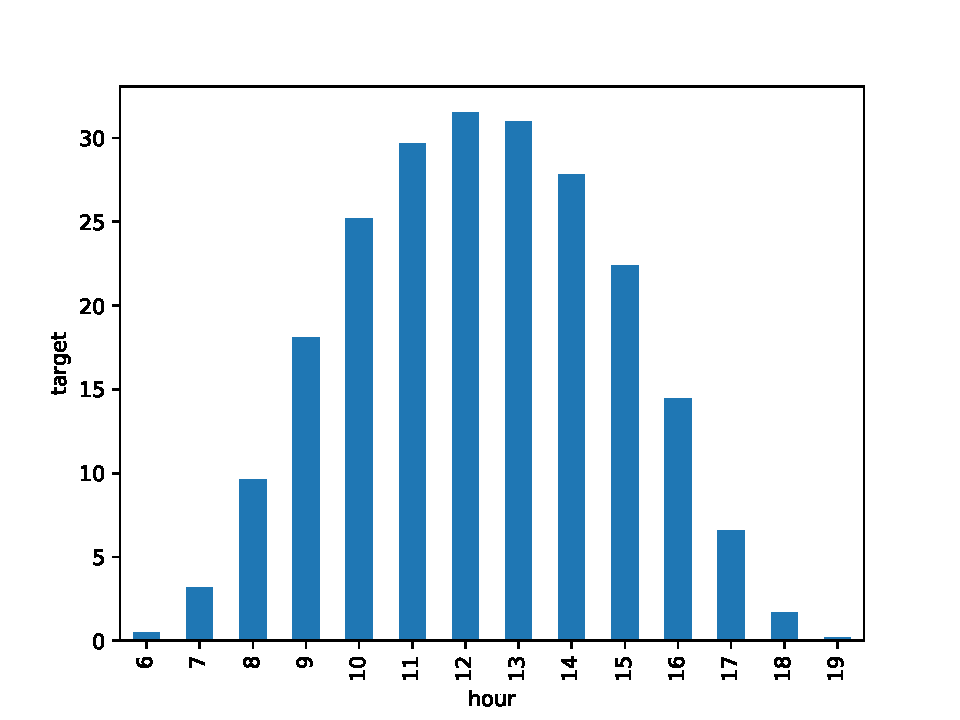
\includegraphics[width=.35 \textwidth]{Chapter4/energies/majorca_groupby_hour_train.pdf}
    \label{fig:maj_groupby_hour}}\quad%
    \subfloat[][]{%
    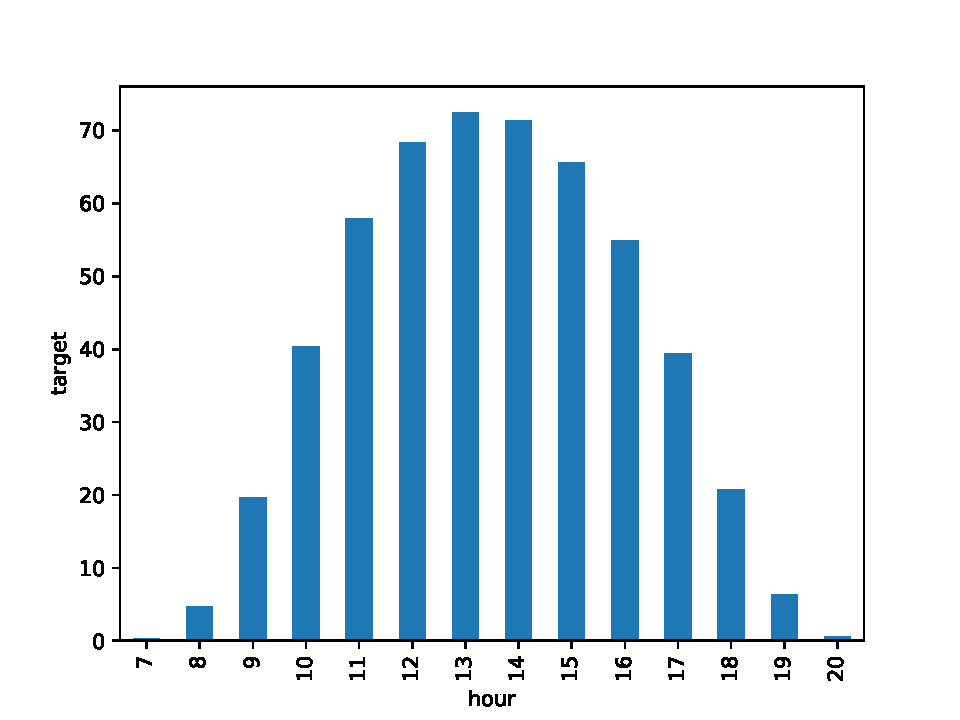
\includegraphics[width=.35 \textwidth]{Chapter4/energies/tenerife_groupby_hour_train.pdf}
    \label{fig:ten_groupby_hour}}\\
    \subfloat[][]{%
    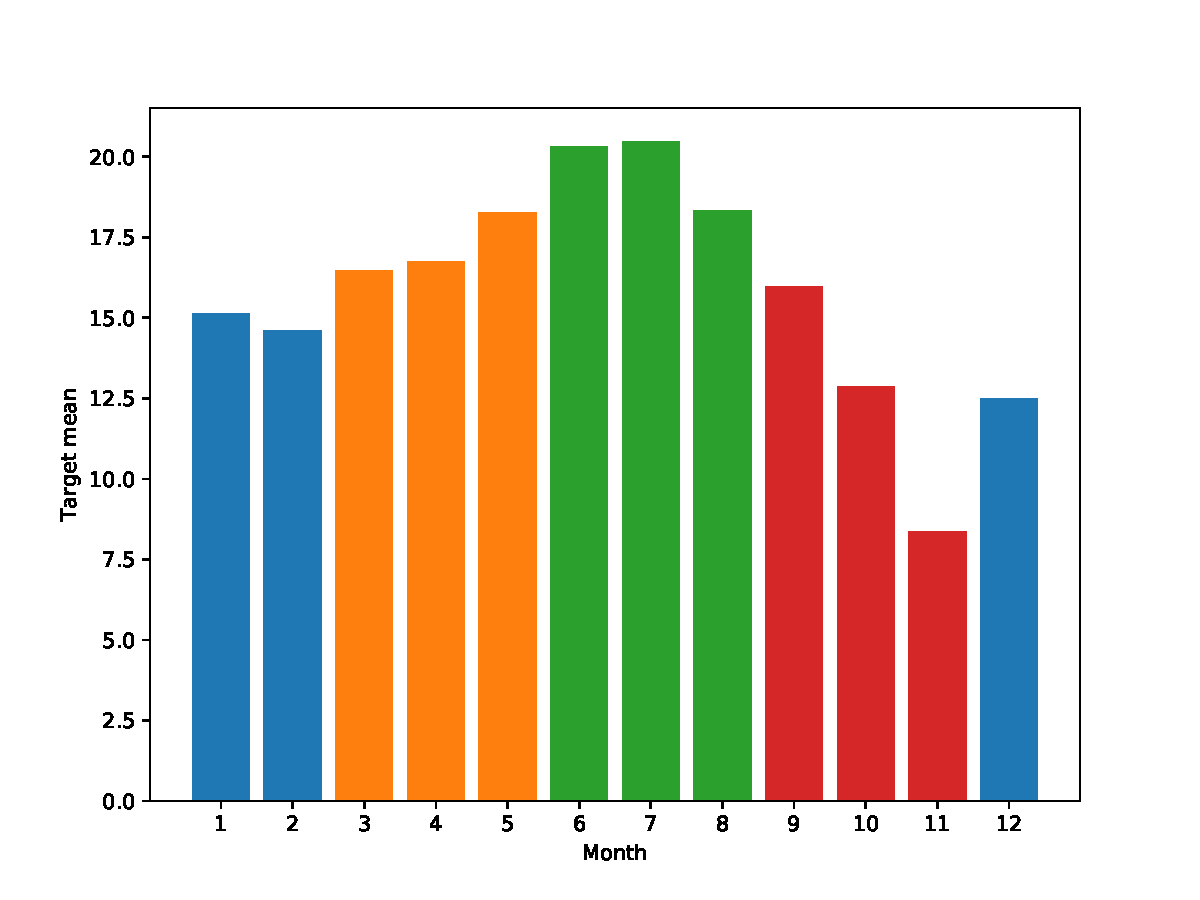
\includegraphics[width=.35 \textwidth]{Chapter4/energies/hist_season_majorca_train_byMonth.pdf}
    \label{fig:maj_groupby_season}}\quad%
    \subfloat[][]{%
    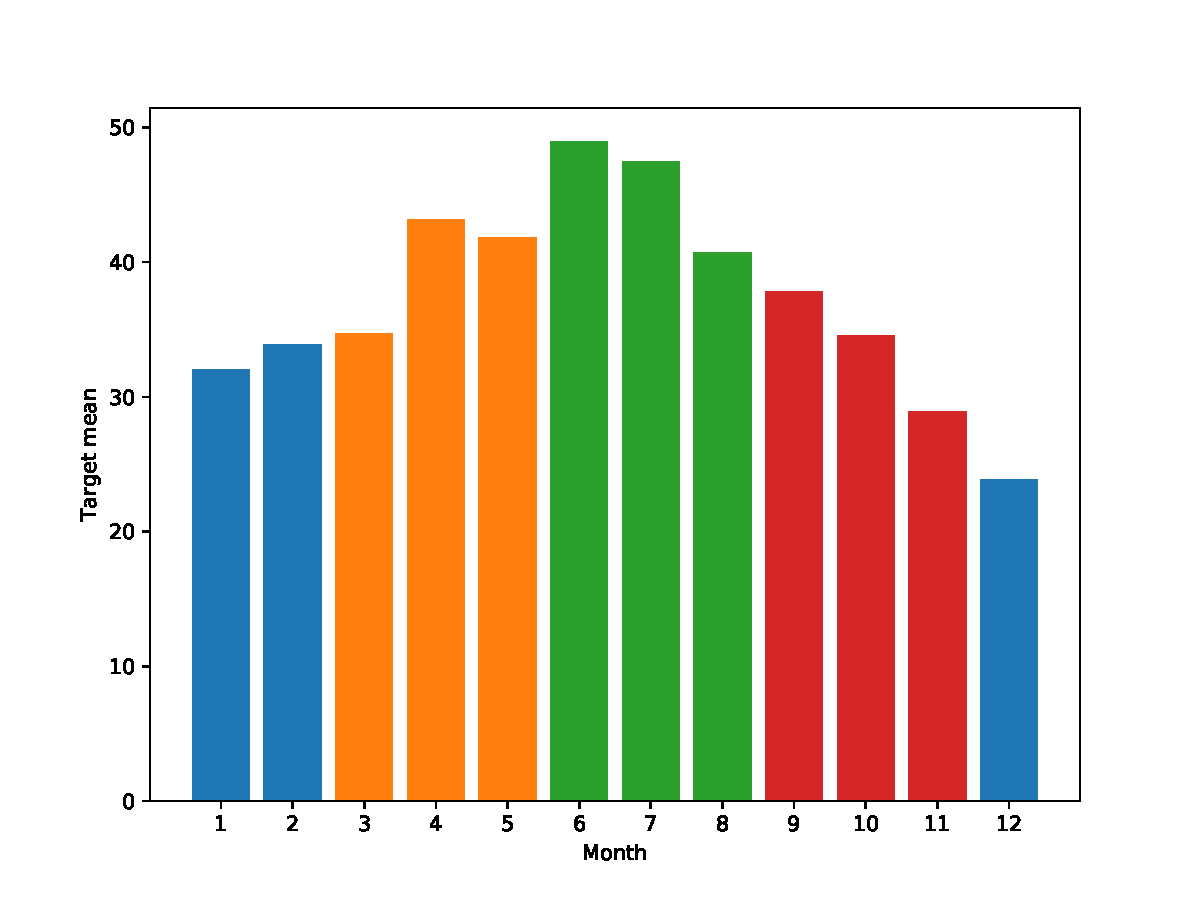
\includegraphics[width=.35 \textwidth]{Chapter4/energies/hist_season_tenerife_train_byMonth.pdf}
    \label{fig:ten_groupby_season}}
 \caption{\label{fig:solar_task_def}Hourly photovoltaic energy mean {in} \fcode{majorca}(~\protect\subref{fig:maj_groupby_hour}) {and}~\fcode{tenerife}(~\protect\subref{fig:ten_groupby_hour}) measured in \mwhu{}. Photovoltaic energy monthly averages for \fcode{majorca}(~\protect\subref{fig:maj_groupby_season}) and \fcode{tenerife}(~\protect\subref{fig:ten_groupby_season}) , colored using the tasks defined using the season and measured in \mwhu{}. All the histograms have been computed using data from year~2016.}
 \end{figure}
 




\paragraph*{Experimental~Results.\\}

\begin{table}[t!]
    \caption{Test MAEs (left), test MSEs (center), with the corresponding rankings, and optimal mixing $\lambda^*$ (right) of the solar energy models considered {in} \fcode{majorca}. {Base units} %Is the bold in the Table necessary? If is not necessary, please remove it. Also, please remove the font in the table. Same as below.
     are either \mwhu{} or percentages (\%). The~best model errors are shown in~bold.}
    \centering
    \label{table:solar_scores_m}
 \begin{tabular}{lccccccc}
    \toprule
     & \fheadmulti{3}{MAE} & \fheadmulti{3}{MSE} & \fhead{$\lambda^*$}\\
    & {{\mwhu}}	& {{\%}} & {rank} & {{\mwhu}}	& {{\textpertenthousand}} & {Rank}& \\
    \midrule
    \fmod{ctlSVR}    &  5.265 &  7.265  & (6) &  59.322 &  112.985  & (6) &  - \\
    \fmod{(season)\_itlSVR}   &  5.305 &  7.384  & (7) &  59.591 &  113.498  & (7) &  - \\
    \fmod{(season)\_mtlSVR}   &  \fmaxn{4.884} &  \fmaxn{6.740}  & \fmaxn{(1)} &  53.222 &  101.366  & (2) &  0.4 \\
    \fmod{(hour)\_itlSVR}   &  5.083 &  7.015  & (4) &  54.540 &  103.877  & (3) &  - \\
    \fmod{(hour)\_mtlSVR}   &  4.957 &  6.840  & (2) &  \fmaxn{52.614} &  \fmaxn{100.208}  & \fmaxn{(1)} &  0.3 \\
    \fmod{(hour, season)\_itlSVR}   &  5.250 &  7.251  & (5) &  57.927 &  110.328  & (5) &  - \\
    \fmod{(hour, season)\_mtlSVR}   &  5.038 &  6.952  & (3) &  54.601 &  103.992  & (4) &  0.3 \\
    \bottomrule
    \end{tabular}
 \end{table}
\unskip


 \begin{table}[t!]
    \caption{Test MAEs (left), test MSEs (center), with the corresponding rankings, and optimal mixing $\lambda^*$ (right) of the solar energy models considered {in} \fcode{tenerife}. Base units are either \mwhu{} or percentages (\%). The~best model errors are shown in~bold. The positions in bold correspond to the model ranked first in terms of MAE or MSE, as indicated by its column.}
    \centering
    \label{table:solar_scores_t}
 \begin{tabular}{lccccccc}
    \toprule
     & \fheadmulti{3}{MAE} & \fheadmulti{3}{MSE} & \fhead{$\lambda^*$}\\
    & {{\mwhu}}	& {{\%}} & {Rank} & {{\mwhu}}	& {{\textpertenthousand}} & {Rank}& \\
    \midrule
    \fmod{ctlSVR}    &  5.786 &  5.373  & (5) &   88.323 &  76.174  & (5) &  - \\
    \fmod{(season)\_itlSVR}   &  5.930 &  5.545  & (6) &   97.454 &  84.611  & (6) &  - \\
    \fmod{(season)\_mtlSVR}   &  5.579 &  5.181  & (4) &   86.227 &  74.366  & (3) &  0.8 \\
    \fmod{(hour)\_itlSVR}   &  5.403 &  5.018  & (2) &   86.686 &  74.762  & (4) &  - \\
    \fmod{(hour)\_mtlSVR}   &  \fmaxn{5.376} &  \fmaxn{4.993}  & \fmaxn{(1)} &   \fmaxn{84.207} &  \fmaxn{72.624}  & \fmaxn{(1)} &  0.7 \\
    \fmod{(hour, season)\_itlSVR}   &  6.025 &  5.554  & (7) &  104.536 &  90.297  & (7) &  - \\
    \fmod{(hour, season)\_mtlSVR}   &  5.494 &  5.102  & (3) &   85.440 &  73.687  & (2) &  0.7 \\
    \bottomrule
    \end{tabular}
 \end{table}
\unskip


\begin{table}[t!]
   \caption{Wilcoxon $p$-values for absolute (left) and quadratic (right) errors.}
   \centering
   \label{table:solar_wilcoxon}
   %% \tablesize{} %% You can specify the fontsize here, e.g.,~\tablesize{\footnotesize}. If commented out \small will be used. Is the bold necessary. Same as others in the table.
   \begin{tabular}{lcccc}
      \toprule
      & \fheadmulti{2}{MAE} &  \fheadmulti{2}{MSE}\\
      & {\fcode{majorca}}	& {\fcode{tenerife}} & {\fcode{majorca}}	& {\fcode{tenerife}}\\
      \midrule
   \fmod{ctlSVR}                           &    0.014 (4) &    0.000 (5) &    0.081 (4) &    0.000 (5) \\
   \fmod{(season)\_itlSVR}                &    0.008 (5) &    0.636 (5) &    0.215 (4) &    0.354 (5) \\
   \fmod{(season)\_mtlSVR}         &   ------ %MDPI: We changed it into minus, please confirm.
{(1)} &    0.000 (4) &    0.036 (2) &    0.000 (3) \\
   \fmod{(hour)\_itlSVR}                  &    0.693 (2) &    0.006 (2) &    0.000 (3) &    0.000 (4) \\
   \fmod{(hour)\_mtlSVR}           &    0.067 (1) &   ------ {(1)} &   ------ {(1)} &   ------ {(1)} \\
   \fmod{(hour, season)\_itlSVR}        &    0.000 (3) &    0.000 (6) &    0.000 (4) &    0.098 (5) \\
   \fmod{(hour, season)\_mtlSVR} &    0.000 (2) &    0.000 (3) &    0.745 (3) &    0.000 (2) \\
   \bottomrule
\end{tabular}
\end{table}

In Tables~\ref{table:solar_scores_m} and~\ref{table:solar_scores_t} we show the numerical results for \fdata{majorca} and \fdata{tenerife}, respectively. We give the test MAE, which is the most natural metric for SVRs, as well as the MSE. 
In the case of percentages, for MAE, we give the percentage corresponding to the total installed power, and for the MSE, the permyriad, that is per \num{10000}, of the installed power.
%
We also show the rankings in terms of MAE or MSE, and the optimal hyperparameter $\lambda^*$ selected by the CV for the \acrshort{mtl} models.
%

To assess statistical significance the Wilcoxon test is used, but instead of testing every pair of models, the rankings of Tables~\ref{table:solar_scores_m} and~\ref{table:solar_scores_t} are used. The Wilcoxon test is applied between each model and the next in ranking at the $0.05$ level, to determine if the difference is significant.
The test is applied over the list of errors commited by each model in the patterns of the test set. When the null hypothesis of the Wilcoxon test is refused, we can assume that the distribution of the difference between the errors does not have its median at $0$.
In Table~\ref{table:solar_wilcoxon}, we show the $p$-values of the pairwise tests. If the $p$-value is smaller than the considered level of 0.05, then the different between models is considered significant.
%
With these procedure, a new significance ranking, shown in Table~\ref{table:solar_wilcoxon},  is generated: starting from the best model, we compare each model with the next best one, and we increase the ranking only if the difference is significant.
%
For example, in Table~\ref{table:solar_scores_m}, in terms of MAE, the first model, \fmod{(season)\_mtlSVR}, is tested against the second one, \fmod{(hour)\_mtlSVR}. In Table~\ref{table:solar_wilcoxon}, we show the $p$-value corresponding to that test, which is $0.067$, and since it is larger than the level $0.05$, the ranking is not increased and we give to both models the same significance ranking. 

%
Looking at the tables, it is easy to see that the \acrshort{mtl} approaches obtain the best results in both problems, while \fmod{ctlSVR} has the worst performance in \fcode{tenerife} and second worst in \fcode{majorca}.
\acrshort{itl} models are more difficult to interpret: although they are always behind their corresponding \acrshort{mtl} approaches, they can obtain good results, see the \fmodt{hour}{itlSVR} in \fdata{majorca} which is second; but they can also have bad performances, as the \fmodt{season}{itlSVR} in \fdata{tenerife}.

%
The $\lambda^*$ values can help to understand this behaviour. In both problems, the selected values lie far from the extremes $0$ or $1$, which distances the \acrshort{mtl} approaches from the \acrshort{ctl} or \acrshort{itl} ones. If these values are optimal, then the \acrshort{ctl} or \acrshort{itl} equivalent models, with $\lambda=1$ and $\lambda=0$, respectively, obtain a worse result in validation. This is reflected also in the test set, as shown in the tables.
Also, it is noticeable that the optimal values for \fdata{majorca} are all smaller than $0.5$, which can be intepreted as models with a stronger common part, while in \fdata{tenerife}, the optimal values are larger than $0.5$ which reflects stronger independent parts.
%
Although the \acrshort{mtl} approaches get the best results with any task definition, the \fmod{(hour)} definition seems to work best than the \fmod{(season)} one. The \fmodt{hour}{mtlSVR} gets a second best result, which is not significantly worse than the best one in \fdata{majorca}, and is the single best result in \fdata{tenerife}.

%
For completeness the scores of persistence models and a neural network are given here.
The persistence forecasts are obtained by predicting at each hour the target value 24 hours prior. By doing this, the MAE scores for \fdata{majorca} and \fdata{tenerife} are \mwh{5.776} and \mwh{7.766}, which scaled to $[0, 100]$ correspond to 7.97\% and 7.21\%; which are an 18\% and 44\% error increase of the best \acrshort{mtl} models.
The neural network errors are \mwh{5.140} and \mwh{5.763}, that is, 7.09\% and 5.35\% of the total \acrshort{pv} installed. While this results are still competitive, this performance is worse than those of the convex \acrshort{mtl} models proposed.


\begin{figure}[t!]
    \centering%
    \subfloat[Best \acrshort{ctl} prediction.]{%
    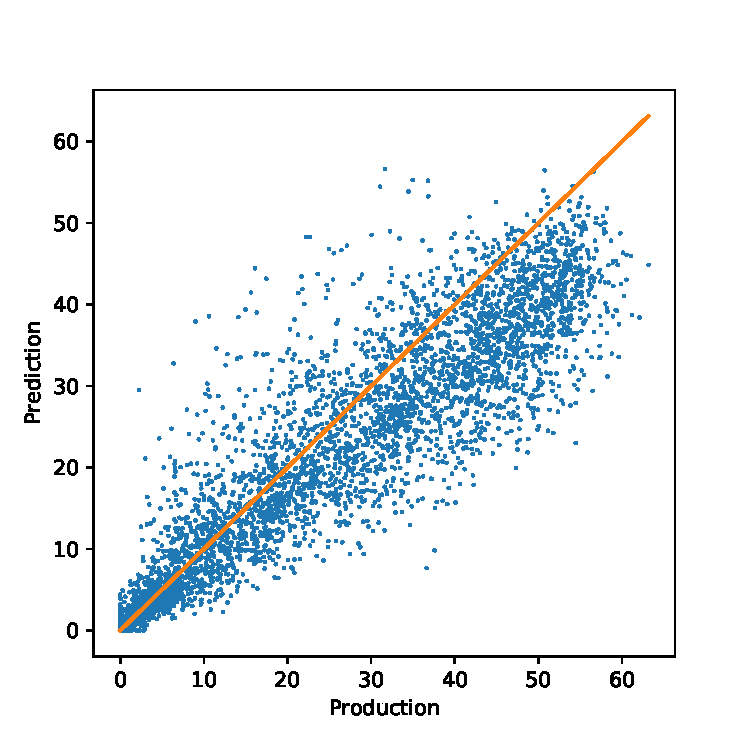
\includegraphics[width=.3 \textwidth, height=.3 \textwidth]{Chapter4/energies/best_ctl_majorca.pdf}
    \label{fig:best_ctl_majorca}}\quad%
    \subfloat[Best \acrshort{itl} prediction.]{%
    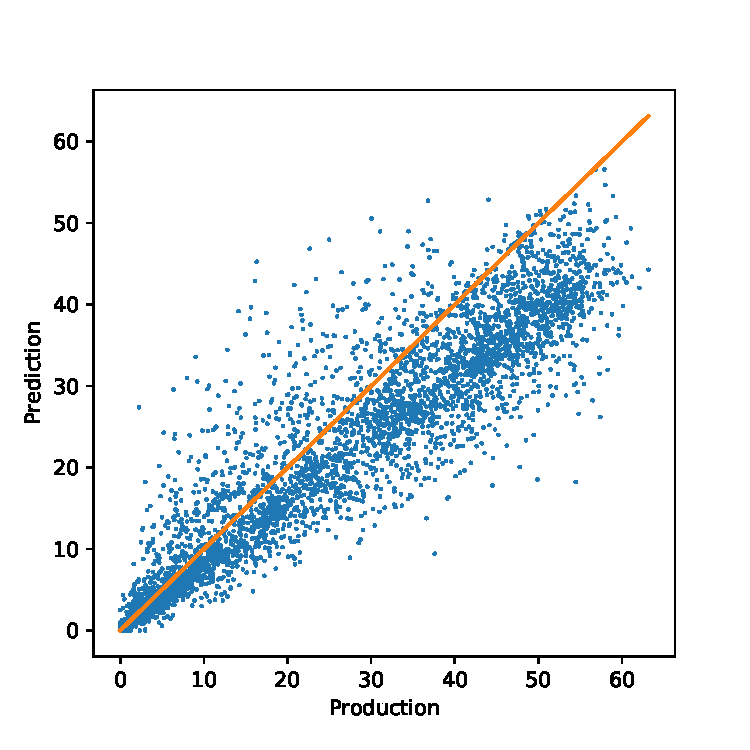
\includegraphics[width=.3 \textwidth, height=.3 \textwidth]{Chapter4/energies/best_itl_majorca.pdf}
    \label{fig:best_itl_majorca}}\quad%
    \subfloat[Best \acrshort{mtl} prediction.]{%
    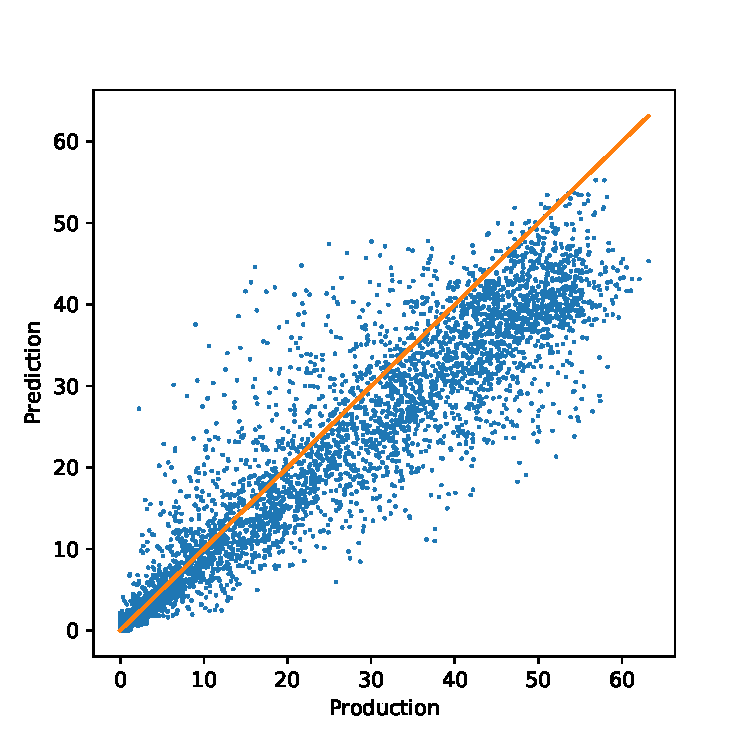
\includegraphics[width=.3 \textwidth, height=.3 \textwidth]{Chapter4/energies/best_mtl_majorca.pdf}
    \label{fig:best_mtl_majorca}}\\
 \caption{\label{fig:majorca_best_plots} Real energy production against the prediction made by the best  models {in} \fcode{majorca}; the perfect prediction line is shown in orange. The~units of the axis are \mwhu{}.}
\end{figure}

\begin{figure}[t!]
    \centering%
    \subfloat[Best \acrshort{ctl} prediction.]{%
    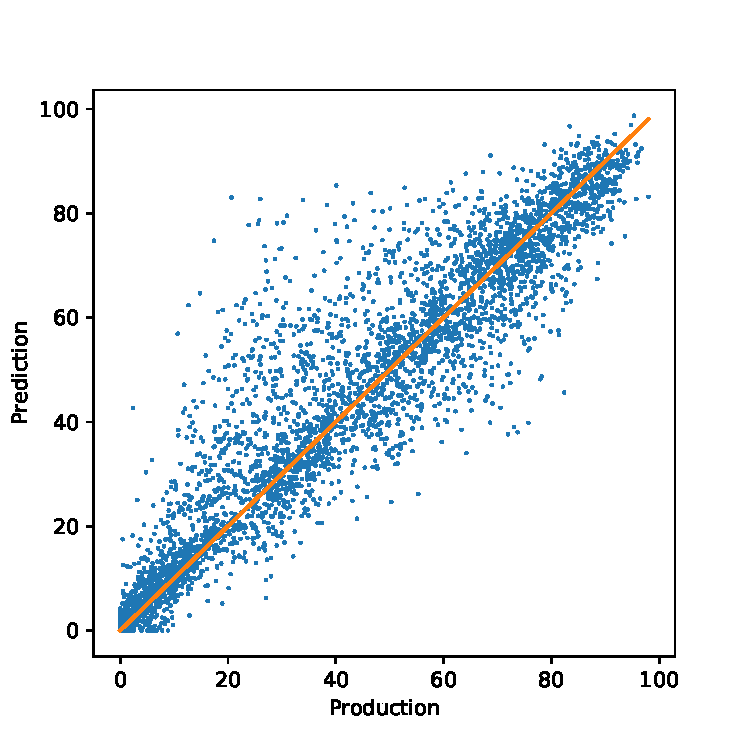
\includegraphics[width=.3 \textwidth, height=.3 \textwidth]{Chapter4/energies/best_ctl_tenerife.pdf}
    \label{fig:best_ctl_tenerife}}\quad%
    \subfloat[Best \acrshort{itl} prediction.]{%
    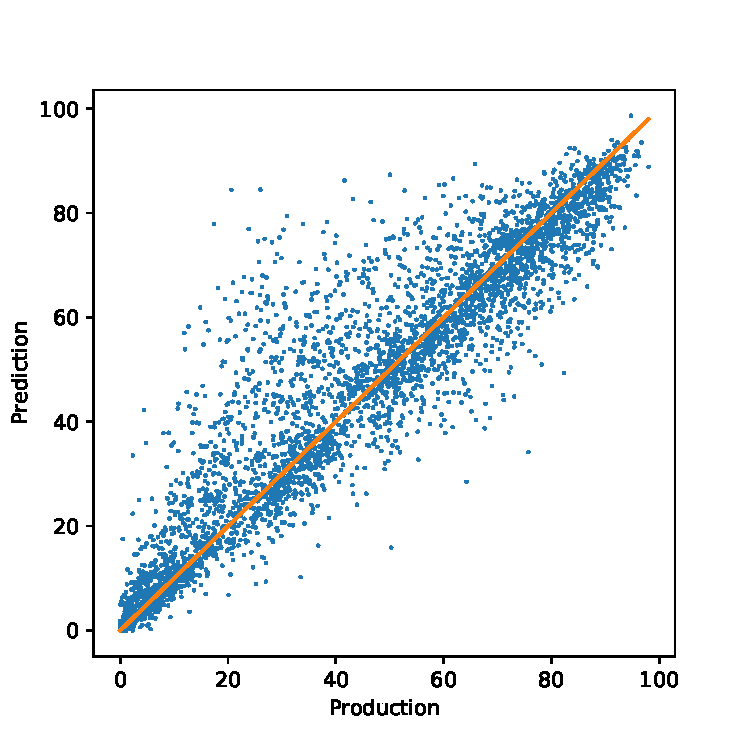
\includegraphics[width=.3 \textwidth, height=.3 \textwidth]{Chapter4/energies/best_itl_tenerife.pdf}
    \label{fig:best_itl_tenerife}}\quad%
    \subfloat[Best \acrshort{mtl} prediction.]{%
    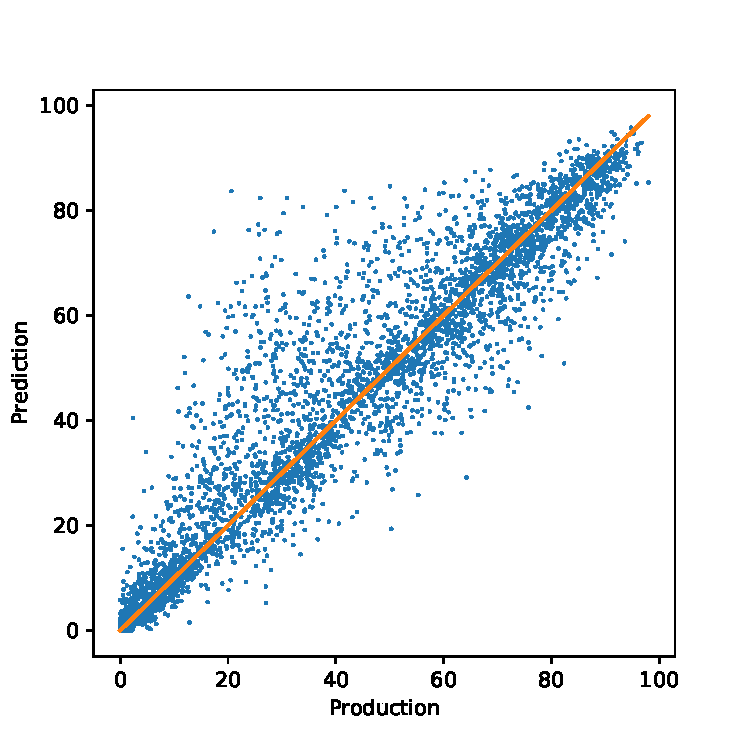
\includegraphics[width=.3 \textwidth, height=.3 \textwidth]{Chapter4/energies/best_mtl_tenerife.pdf}
    \label{fig:best_mtl_tenerife}}\\
 \caption{\label{fig:tenerife_best_plots} Real energy production against prediction made by the best models {in} \fcode{tenerife}; the perfect prediction  line is shown in orange. The~units of the axis are \mwhu{}.}
\end{figure}


%
To get a better understanding of the results we plot the predictions against the target values of the \acrshort{ctl} model and the best \acrshort{itl} and \acrshort{mtl} ones.
%
In the case of \fdata{majorca}, we plot the predictions \fmod{ctlSVR}, \fmodt{hour}{itlSVR} and \fmodt{season}{mtlSVR} in Figure~\ref{fig:majorca_best_plots}.
From these scatter plots it seems that the \acrshort{ctl} approach has a larger deviation in its predictions, while the \acrshort{itl} one has a bias, that is, it systematically underestimates the prediction corresponding to larger values of energy production.
The \acrshort{mtl} approach seems to correct, to a certain degree, this bias of the \acrshort{itl} model, while preserving a smaller variance than the \acrshort{ctl} one.
%
For \fdata{tenerife} we plot the predictions of \fmod{ctlSVR}, \fmodt{hour}{itlSVR} and \fmodt{hour}{mtlSVR}, which are shown in Figure~\ref{fig:tenerife_best_plots}.
It is more difficult to interpret the plots in this case, although it is possible to highlight that the \acrshort{mtl} approach seems less prone to overestimate the production at lower values than either the \acrshort{ctl} or \acrshort{itl} models.







\subsection{Wind Energy}
We want to predict the wind energy production at the Sotavento wind park located in Galicia, Spain.
Wind energy forecasting is more challenging than the photovoltaic one, due to the unstable nature of the wind, whose behavior is more chaotic than solar radiation. Detecting scenarios where the wind energy production behaves differently but is stable in each one seems crucial, but it is a difficult task. Looking at different characteristics of wind energy production we establish some task definitions and use them to test our proposal. 

\paragraph*{Data and~Tasks.\\}

\begin{figure}[t!]
    \centering%
    \subfloat[Histogram of wind angles colored by task definition \fmod{angle}.]{%
    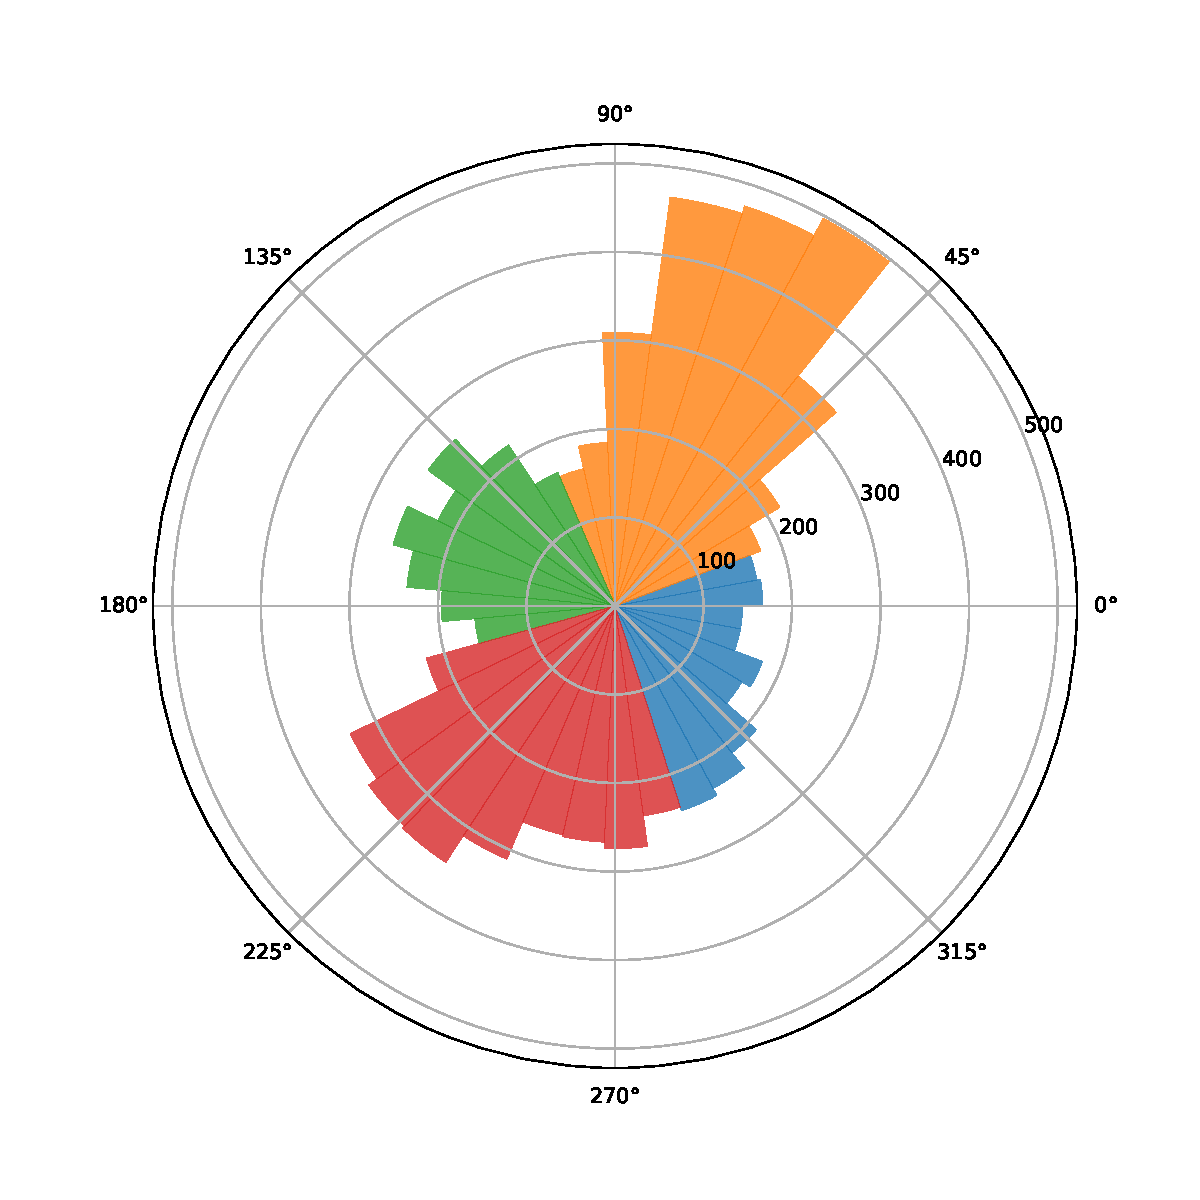
\includegraphics[width=.38 \textwidth]{Chapter4/energies/polarhist_tasks_angle_stv_train.pdf}
    \label{fig:stv_task_angle}}\quad%
    \subfloat[Histogram of wind velocity (\si{\metre/\second}) in Sotavento colored by {task} definition \fmod{velocity}.]{%
    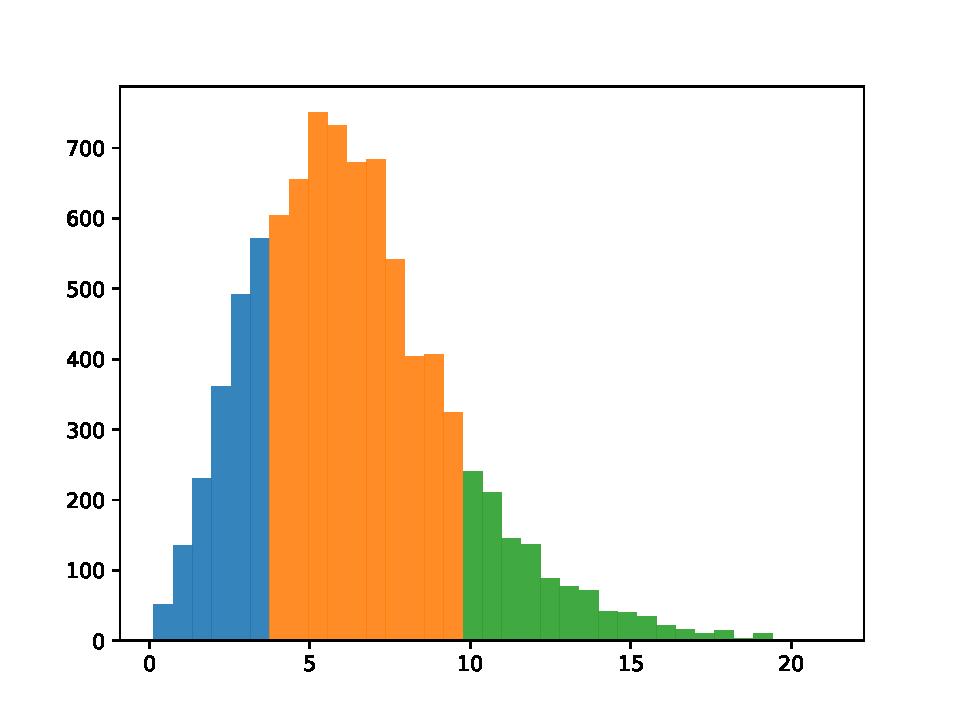
\includegraphics[width=.38 \textwidth]{Chapter4/energies/hist_tasks_velocity_stv_train.pdf}
    \label{fig:stv_task_velocity}}\\
 \caption{\label{fig:wind_task_def} Histograms of wind derived from NWP data for the year 2016 in Sotavento.}
\end{figure}

 \begin{figure}[t!]
   \centering
   \subfloat[{Hourly mean measured} of generated energy (\si{\kilo{\watt\hour}}) colored by {task} definition \fmod{timeOfDay}.]{%
   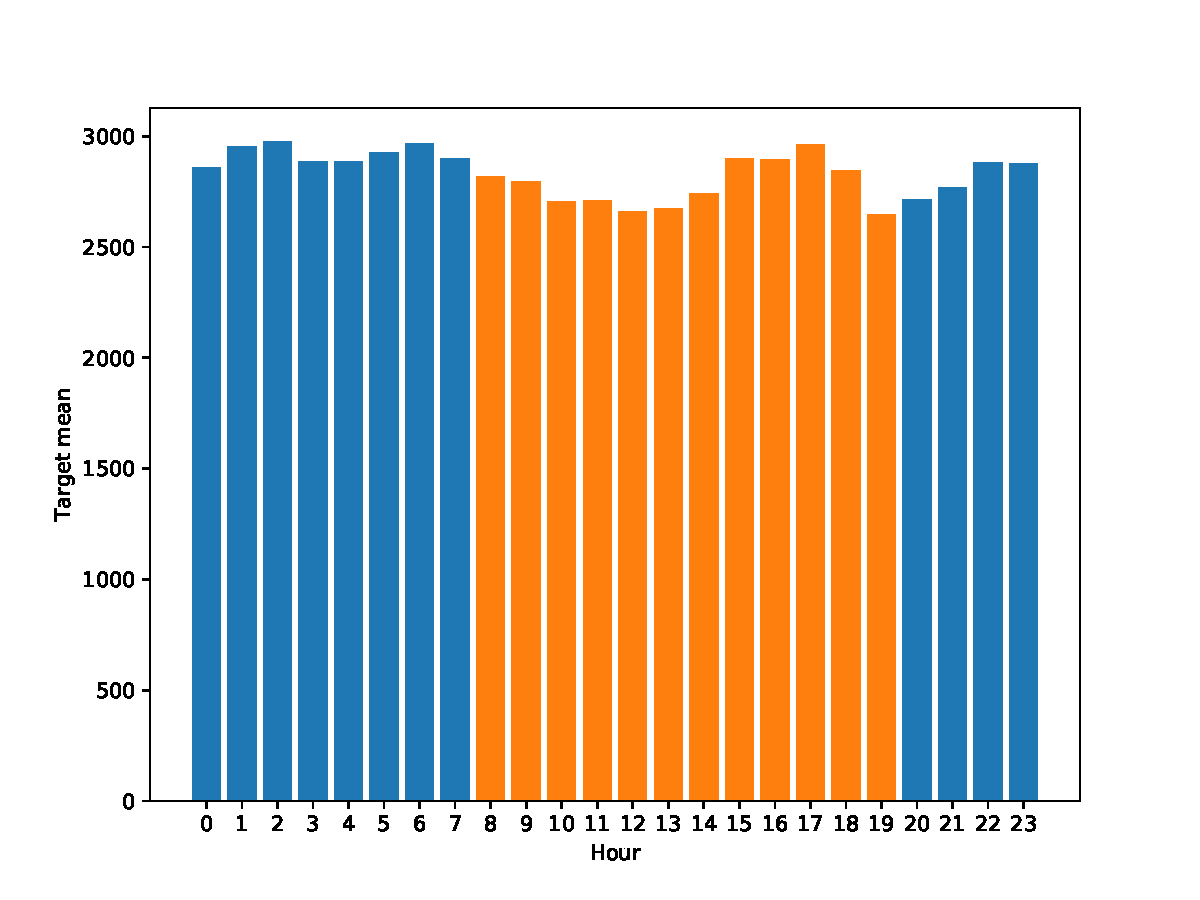
\includegraphics[width=.45 \textwidth]{Chapter4/energies/hist_timeOfDay_stv_train_byHour.pdf}
   \label{fig:hist_timeOfDay_stv_target}}%
\subfloat[Hourly mean of velocity (\si{\metre/\second}) at \SI{100}{\metre} colored by {task} definition \fmod{timeOfDay}.]{%
    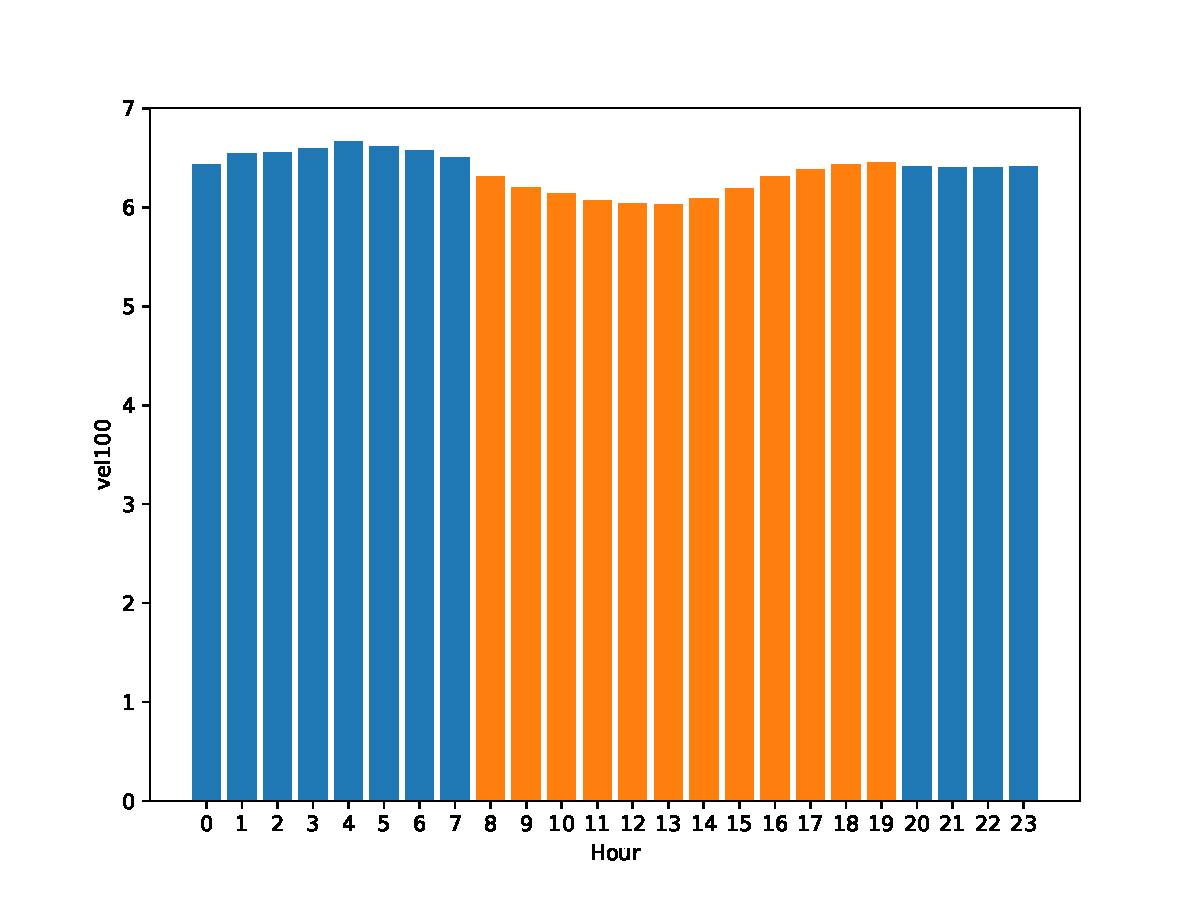
\includegraphics[width=.45 \textwidth]{Chapter4/energies/hist_timeOfDay_stv_vel100_byHour.pdf}
    \label{fig:hist_timeOfDay_stv_vel100}}
% \hspace{\fill}
\caption{\label{fig:wind_task_def} Histograms of wind derived from NWP data for the year 2016 in Sotavento.}
\end{figure}

\begin{figure}[t!]
   \centering
   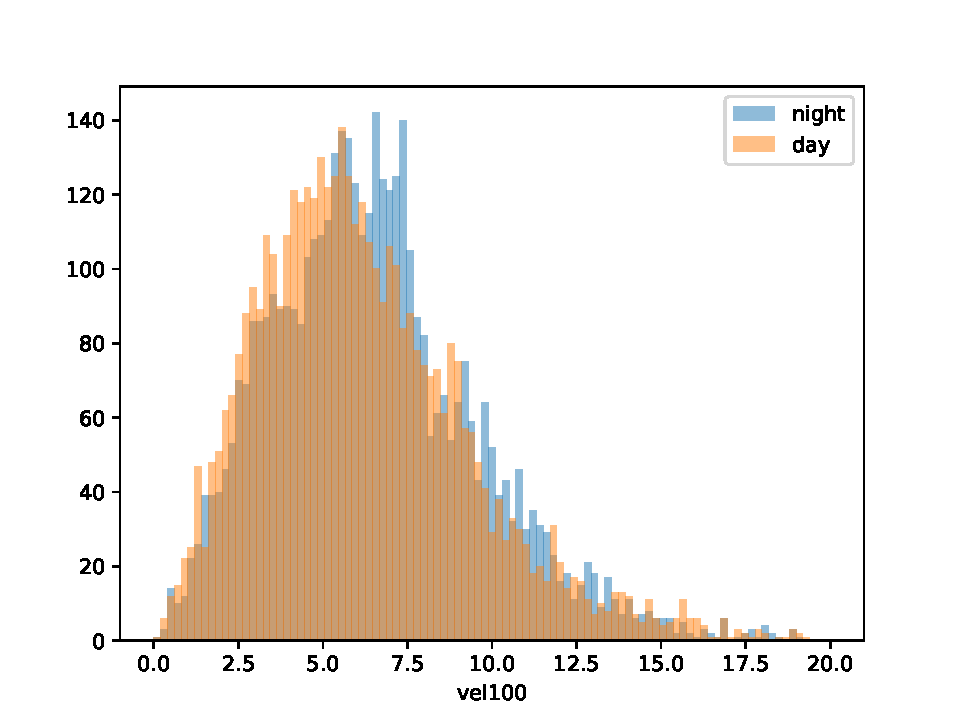
\includegraphics[width=.5\textwidth]{Chapter4/energies/hist_timeOfDay_stv_vel100_normal.pdf}
 \caption{\label{fig:stv_vel100} Histograms of the velocity of wind at 100m derived from NWP data for the year 2016 and measured in m/s during the day and night in Sotavento.
%  \comm{decir para qué año. Hay una cosa que no entiendo: a ojo parece que hay más datos de night que de day, lo que no debería ser. Pero mirando la fig anterior hay 11 horas night-azul- y 13 day naranja. Claramente está mal, pero así las cosas los colores de abajo están al revés}
}
\end{figure}

The variables from the NWP that we consider as predictors are:
\begin{itemize}
    \item	Eastward component of the wind at {10 m} %Please remove the font. Same as below
     (\ftt{U10}).
    \item	Northward  component of the wind at {10 m} (\ftt{V10}).
    \item   Module of velocity of the wind at 10 m (\ftt{vel10}).
    \item	Eastward  component of the wind at {100 m} (\ftt{U100}).
    \item	Northward component of the wind at {100 m} (\ftt{V100}).
    \item   Module of velocity of the wind at 100 m (\ftt{vel100}).
    \item   Surface {Pressure} (\ftt{sp}).
    \item	2 meter {temperature} (\ftt{2t}).
\end{itemize}
These variables are collected in a grid, which is approximately centered at the farm, with northwest and southeast coordinates at $(\ang{-9.5}, \ang{44})$ and $(\ang{-6}, \ang{42.25})$, respectively, and a spatial resolution of $\ang{0.125}$.
This results in a grid with $435$ points, that, with the $8$ variables considered at each point, gives a total number of {3480} predictive features.
We scale the energy productions values to $[0, 100]$ using the maximum power installed (\mw{17.56}), which corresponds to the value $100$.
%
Recall that we have three years of data, 2016, 2017 and 2018, which are used as train, validation and test sets.
%
Although there are no obvious task definitions, we consider three different criteria:
\begin{itemize}
    \item \fmod{angle}: Here the wind angle at a height of \si{100\metre} is considered, which is obtained from the \ftt{U100} and \ftt{V100} variables. 
    First, the most frequent angle is estimated, which is $\ang{56}$, and then, we use it as the center of the first quadrant. That is, the patterns that correspond to the first task as those whose wind angle lies between ${11}$ and $\ang{101}$  The other three quadrants, corresponding to a task each, are defined by the remaining sectors of $\ang{90}$.
    The histogram of wind angles, and the defined quadrants in different colors, are shown in Figure~\ref{fig:stv_task_angle}.
    \item \fmod{velocity}: Here the wind velocity at a height of \si{100\metre} is considered, which is again obtained from the \ftt{U100} and \ftt{V100} variables. The speed boundaries selected to define three tasks are $4$ and $10$m/s, which, for an ideal generator, are approximately the starting point of wind energy generation and its maximum power plateau, before cut-off speed.   
    In Figure~\ref{fig:stv_task_velocity} the histrogram of velocities is shown with the task regions colored. 
    \item \fmod{timeOfDay}: Here the 24 hours of a day are divided in two 12 hours periods: a day period between 08 and \utc{19}, and~a night one between 20 to \utc{07}.
    In Figures~\ref{fig:hist_timeOfDay_stv_target} and~\ref{fig:hist_timeOfDay_stv_vel100} the hourly average energy production and wind speed are shown, with the hours colored according to the two tasks defined. In Figure~\ref{fig:stv_vel100} the histograms of wind velocity in the night and day periods are shown.
\end{itemize}
%
For these task definitions, it is necessary to perform an analysis of the data, which is done only using the train set, corresponding to 2016.
The tasks in this case are not as clear as those defined for the solar energy. For the \fmod{angle} and \fmod{velocity} definitions some differences across tasks in the histograms can be found, but not definitive ones.
For the \fmod{timeOfDay} definition, the two histograms of Figure~\ref{fig:stv_vel100} look very similar.
Moreover, the boundaries of the tasks are set in a way that is partially arbitrary, and a bad selection of tasks could lead to poor results.


\paragraph*{Experimental~Results.\\}


\begin{table}[t!]
    \caption{Test MAEs (left), {MSEs} %Please remove the font in the table. Same in Table 6.
     scores (center), with the corresponding rankings, and optimal mixing $\lambda^*$ (right) of the Sotavento wind energy models considered. The~best model errors are shown in~bold.}
    \centering
    \label{table:wind_scores}
    %% \tablesize{} %% You can specify the fontsize here, e.g.,~\tablesize{\footnotesize}. If commented out \small will be used.
    \begin{tabular}{lccc}
    \toprule
    & \fhead{MAE} &  \fhead{MSE} &  \fhead{$\lambda^*$}\\
%    & \fhead{\fcode{stv}}	& \fhead{\fcode{stv}} & \fhead{\fcode{stv}} \\
    \midrule
    \fmod{ctlSVR}                                           &   \fmaxn{6.132} (1) &    90.228 (2) & - \\
    \fmod{(velocity)\_itlSVR}                              &  6.211 (7) &   93.363 (7) & - \\
    \fmod{(velocity)\_mtlSVR}                       &   6.208 (6) &    93.199 (6) & 0 \\
    \fmod{(timeOfDay)\_itlSVR}                             &  6.283 (9) &   93.594 (9) & - \\
    \fmod{(timeOfDay)\_mtlSVR}                      &   \fmaxn{6.132} (1) &    90.228 (2) & 1 \\
    \fmod{(timeOfDay, velocity)\_itlSVR}                 &  6.341 (11) &   97.250 (11) & - \\
    \fmod{(timeOfDay, velocity)\_mtlSVR}          &  6.312 (10) &   94.774 (10) & 0.4 \\
    \fmod{(timeOfDay, angle)\_itlSVR}                    &  6.266 (8) &   93.517 (8) & - \\
    \fmod{(timeOfDay, angle)\_mtlSVR}             &   \fmaxn{6.132} (1) &    90.228 (2) & 1 \\
    \fmod{(timeOfDay, angle, velocity)\_itlSVR}        &  6.410 (12) &  102.031 (12) & - \\
    \fmod{(timeOfDay, angle, velocity)\_mtlSVR} &   \fmaxn{6.132} (1) &    90.228 (2) & 1 \\
    \fmod{(angle)\_itlSVR}                                 &   6.170 (4) &    91.586 (4) & - \\
    \fmod{(angle)\_mtlSVR}                          &   6.135 (2) &    \fmaxn{90.026} (1) & 0.9 \\
    \fmod{(angle, velocity)\_itlSVR}                     &   6.173 (5) &    92.529 (5) & - \\
    \fmod{(angle, velocity)\_mtlSVR}              &   6.168 (3) &    90.990 (3) & 0.7 \\
    \bottomrule
    \end{tabular}
\end{table}



\begin{table}[t!]
    \caption{Wilcoxon $p$-values and {corresponding} %Please add explanations of ``—''. In addition, please remove bold if appropritate.
     rankings for absolute (right) and square (left) wind energy errors in~Sotavento. The positions in bold correspond to the model ranked first in terms of MAE or MSE, as indicated by its column.}
    \centering
    \label{table:wind_wilcoxon}
    %% \tablesize{} %% You can specify the fontsize here, e.g.,~\tablesize{\footnotesize}. If commented out \small will be used.
    \begin{tabular}{lcc}
    \toprule
    & \fhead{MAE} &  \fhead{MSE}\\
%    & \fhead{\fcode{stv}}	& \fhead{\fcode{stv}} \\
    \midrule
\fmod{ctlSVR}                                           &     ------  {(1)} &    ------   (2)  \\
\fmod{(velocity)\_itlSVR}                              &    0.570  (3) &    0.150  (3)  \\
\fmod{(velocity)\_mtlSVR}                       &    0.356  (3) &    0.466 (3)  \\
\fmod{(timeOfDay)\_itlSVR}                             &    0.195  (4) &    0.258  (4)  \\
\fmod{(timeOfDay)\_mtlSVR}                      &      ------   {(1)} &      ------   (2)  \\
\fmod{(timeOfDay, velocity)\_itlSVR}                 &    0.941  (4) &    0.021  (5)  \\
\fmod{(timeOfDay, velocity)\_mtlSVR}          &    0.428  (4) &    0.650 (4)  \\
\fmod{(timeOfDay, angle)\_itlSVR}                    &    0.000  (4) &    0.015  (4)  \\
\fmod{(timeOfDay, angle)\_mtlSVR}             &      ------   {(1)} &      ------   (2)  \\
\fmod{(timeOfDay, angle, velocity)\_itlSVR}        &    0.090  (4) &    0.024  (6)  \\
\fmod{(timeOfDay, angle, velocity)\_mtlSVR} &   ------  {(1)} &    ------   (2)  \\
\fmod{(angle)\_itlSVR}                                 &    0.855  (3) &    0.644  (3)  \\
\fmod{(angle)\_mtlSVR}                          &    0.035  (2) &   ------  {(1)} \\
\fmod{(angle, velocity)\_itlSVR}                     &    0.253  (3) &    0.465  (3)  \\
\fmod{(angle, velocity)\_mtlSVR}              &    0.018  (3) &    0.001 (3)   \\
\bottomrule
    \end{tabular}
\end{table}

In Table~\ref{table:wind_scores} the MAE and MSE scores are shown, and also the ranking is given in parentheses. 
Unlike the solar energy case, here the \acrshort{ctl} approach seems better suited than using an \acrshort{itl} one. This is also reflected in the selection of $\lambda^*$ values in the models that get best results, which are close to $1$, the \acrshort{ctl} equivalent case. That is \acrshort{mtl} models such as \fmodt{timeOfDay}{mtlSVR}, \fmodt{timeOfDay, angle}{mtlSVR} and \fmodt{timeOfDay, angle, velocity}{mtlSVR}, where $\lambda^*=1$, obtain the best results and are equivalent to \fmod{ctlSVR}. Also note the cases of \fmodt{angle}{mtlSVR} and \fmodt{angle, velocity}{mtlSVR}, that are second and third, and where the selected values are $\lambda^*=0.9$ and $\lambda^*=0.7$.
Those models that put the emphasis on the independent parts, like \fmodt{timeOfDay, velocity}{mtlSVR}, and, of course, the \acrshort{itl} approaches, get worse results.
%
%
As with the solar energy problems, the statistical significance of the results is tested using the Wilcoxon test. As before, using the ranking of Table~\ref{table:wind_scores}, the significance of the difference between one model and its immediate succesor is tested. 
%
In Table~\ref{table:wind_wilcoxon} the $p$-values of these Wilcoxon tests are given, and the statistical significance ranking is shown. Recall that two models have different significance ranking only if the Wilcoxon test hypothesis is refused.
%
The \acrshort{ctl} approach obtains the best results, being the best model in terms of MAE and second best in terms of MSE. Nevertheless, the equivalent \acrshort{mtl} approaches that use $\lambda^*=1$ trivially tie at first place; these are \fmodt{timeOfDay}{mtlSVR}, \fmodt{timeOfDay, angle}{mtlSVR} and \fmodt{timeOfDay, angle, velocity}{mtlSVR}, while the \fmodt{angle}{mtlSVR} gets the second best MAE score.
When the MSE scores are analyzed, the roles are reversed, the \fmodt{angle}{mtlSVR} gets the best result, and the \fmod{ctlSVR} and the equivalents \acrshort{mtl} approaches are second.

%
This advantage of the \acrshort{ctl} approach can find its roots on poorly defined tasks, which do not have a strong relation with the energy production. Also, the definition of the tasks is made using the train set, data from year 2016, which may not be useful to the validation or test years.
Nevertheless, the \acrshort{mtl} approaches, having the possibility of blending to either \acrshort{ctl} or \acrshort{itl} approaches get the best results too.

%
In this wind energy problem, the persistence forecasts, which again predict the energy production the previous day at the same hour, obtain an error of $15.64\%$, which is quite large and represent a $150\%$ increase on the lowest error using SVRs. This is not unusual, since the wind velocity or angle between two different days are not necessarily correlated.
%
With the neural network regressor, the error is a $6.66\%$, which is also greater than any of the models considered.

\begin{figure}[t!]
    \centering%
    \subfloat[Best \acrshort{ctl} prediction.]{%
    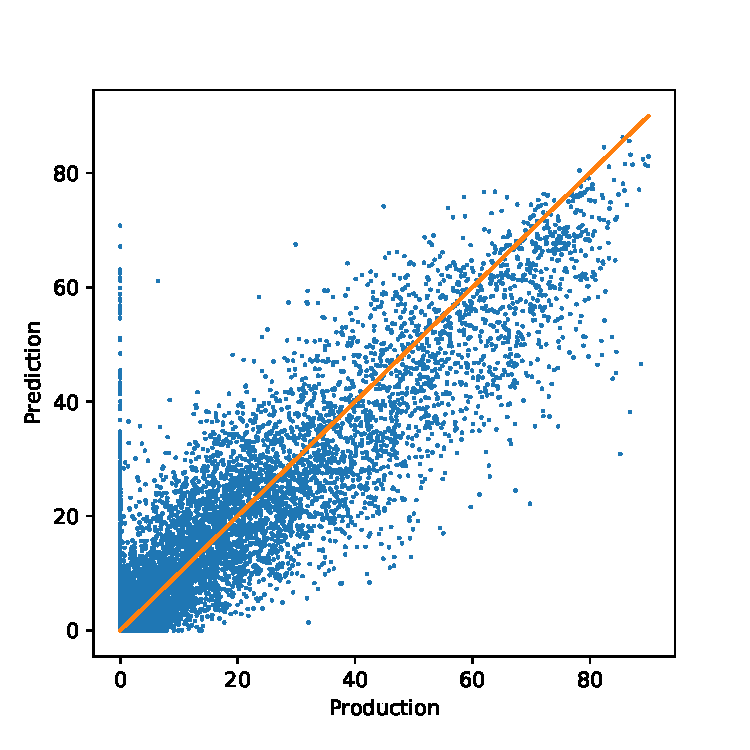
\includegraphics[width=.3 \textwidth, height=.3 \textwidth]{Chapter4/energies/best_ctl_stv.pdf}
    \label{fig:best_ctl_stv}}\quad%
    \subfloat[Best \acrshort{itl} prediction.]{%
    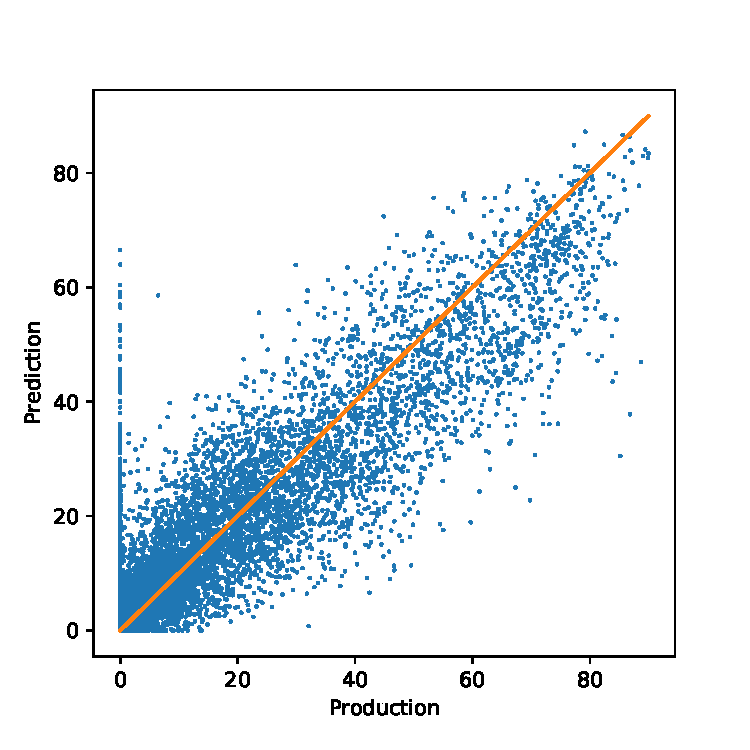
\includegraphics[width=.3 \textwidth, height=.3 \textwidth]{Chapter4/energies/best_itl_stv.pdf}
    \label{fig:best_itl_stv}}\quad%
    \subfloat[Best \acrshort{mtl} prediction.]{%
    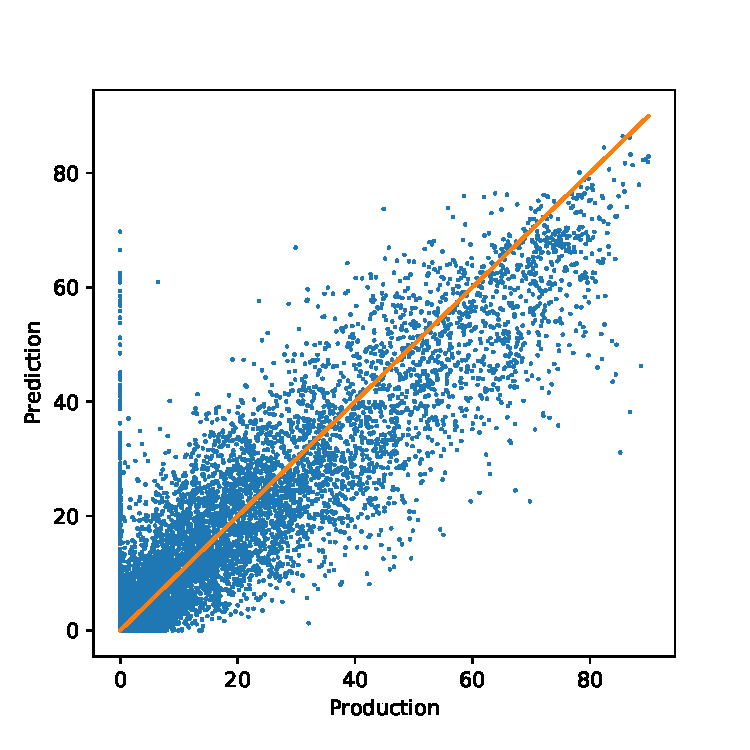
\includegraphics[width=.3 \textwidth, height=.3 \textwidth]{Chapter4/energies/best_mtl_stv.pdf}
    \label{fig:best_mtl_stv}}\\
 \caption{\label{fig:stv_best_plots} Real energy production against prediction made by the best models for \fdata{sotavento}; the perfect prediction line is shown in orange. The~units of the axis are percentages points of the total \acrshort{pv} energy~installed.}
 \end{figure}

%
Again, we plot the predictions agains the target values of the \acrshort{ctl} model and best \acrshort{itl},~\fmodt{angle}{itlSVR}, and pure \acrshort{mtl}, \fmodt{angle}{mtlSVR} approaches.
The presence of points with zero production is noticeable, but this is relatively frequent in wind energy. It can be caused either by energy curtailments or by maintenance periods of the wind farm.
Also, it is appreciable the frequency of small production values, below \SI{20}{\percent}, which is due to the approximate Weibull distribution of wind speeds, where small speed values have higher frequencies. 
With these considerations, it is difficult to compare the plots and find significant differences in model performance.







% \subsection{Conclusions}

% \paragraph*{old\\}%

% We finally observe that while the wind MAEs in percentage are similar to those in \acrshort{pv}, when compared with the energy produced, the~performance of wind models is actually worse.
% In fact, in~Table~\ref{table:comparison} we compare the percentage MAE against the average generated energy as a percentage of installed power.
% As~it can be seen, the~ratio between the percentage MAE and the percentage average energy is about $34.78\%$ for Sotavento, much higher than the $22.50\%$ of Majorca and the $14.92\%$ of~Tenerife.

% \begin{table}[t!]
%     \caption{{Comparison}        %Please remove font in the Table
%      of the percentage MAEs with the average energy produced as a percentage of installed~power.}
%     \centering
%     \label{table:comparison}
%     %% \tablesize{} %% You can specify the fontsize here, e.g.,~\tablesize{\footnotesize}. If commented out \small will be used.
%     \begin{tabular}{lccc}
%     \toprule
%  & \fhead{MAE (\%)} & \fhead{Avg. Target (\%)} & \fhead{Ratio} \\
% 	\midrule
% \fdata{majorca} & 6.740 & 29.954 & 22.50 \\
% \fdata{tenerife} & 4.993 & 33.462 & 14.92 \\
% \fdata{sotavento} & 6.186	& 17.784 & 34.78 \\
% \bottomrule
%     \end{tabular}
% \end{table}













































\section{Convex Multi-Task Learning with Neural Networks}

\begin{figure}[t!]
    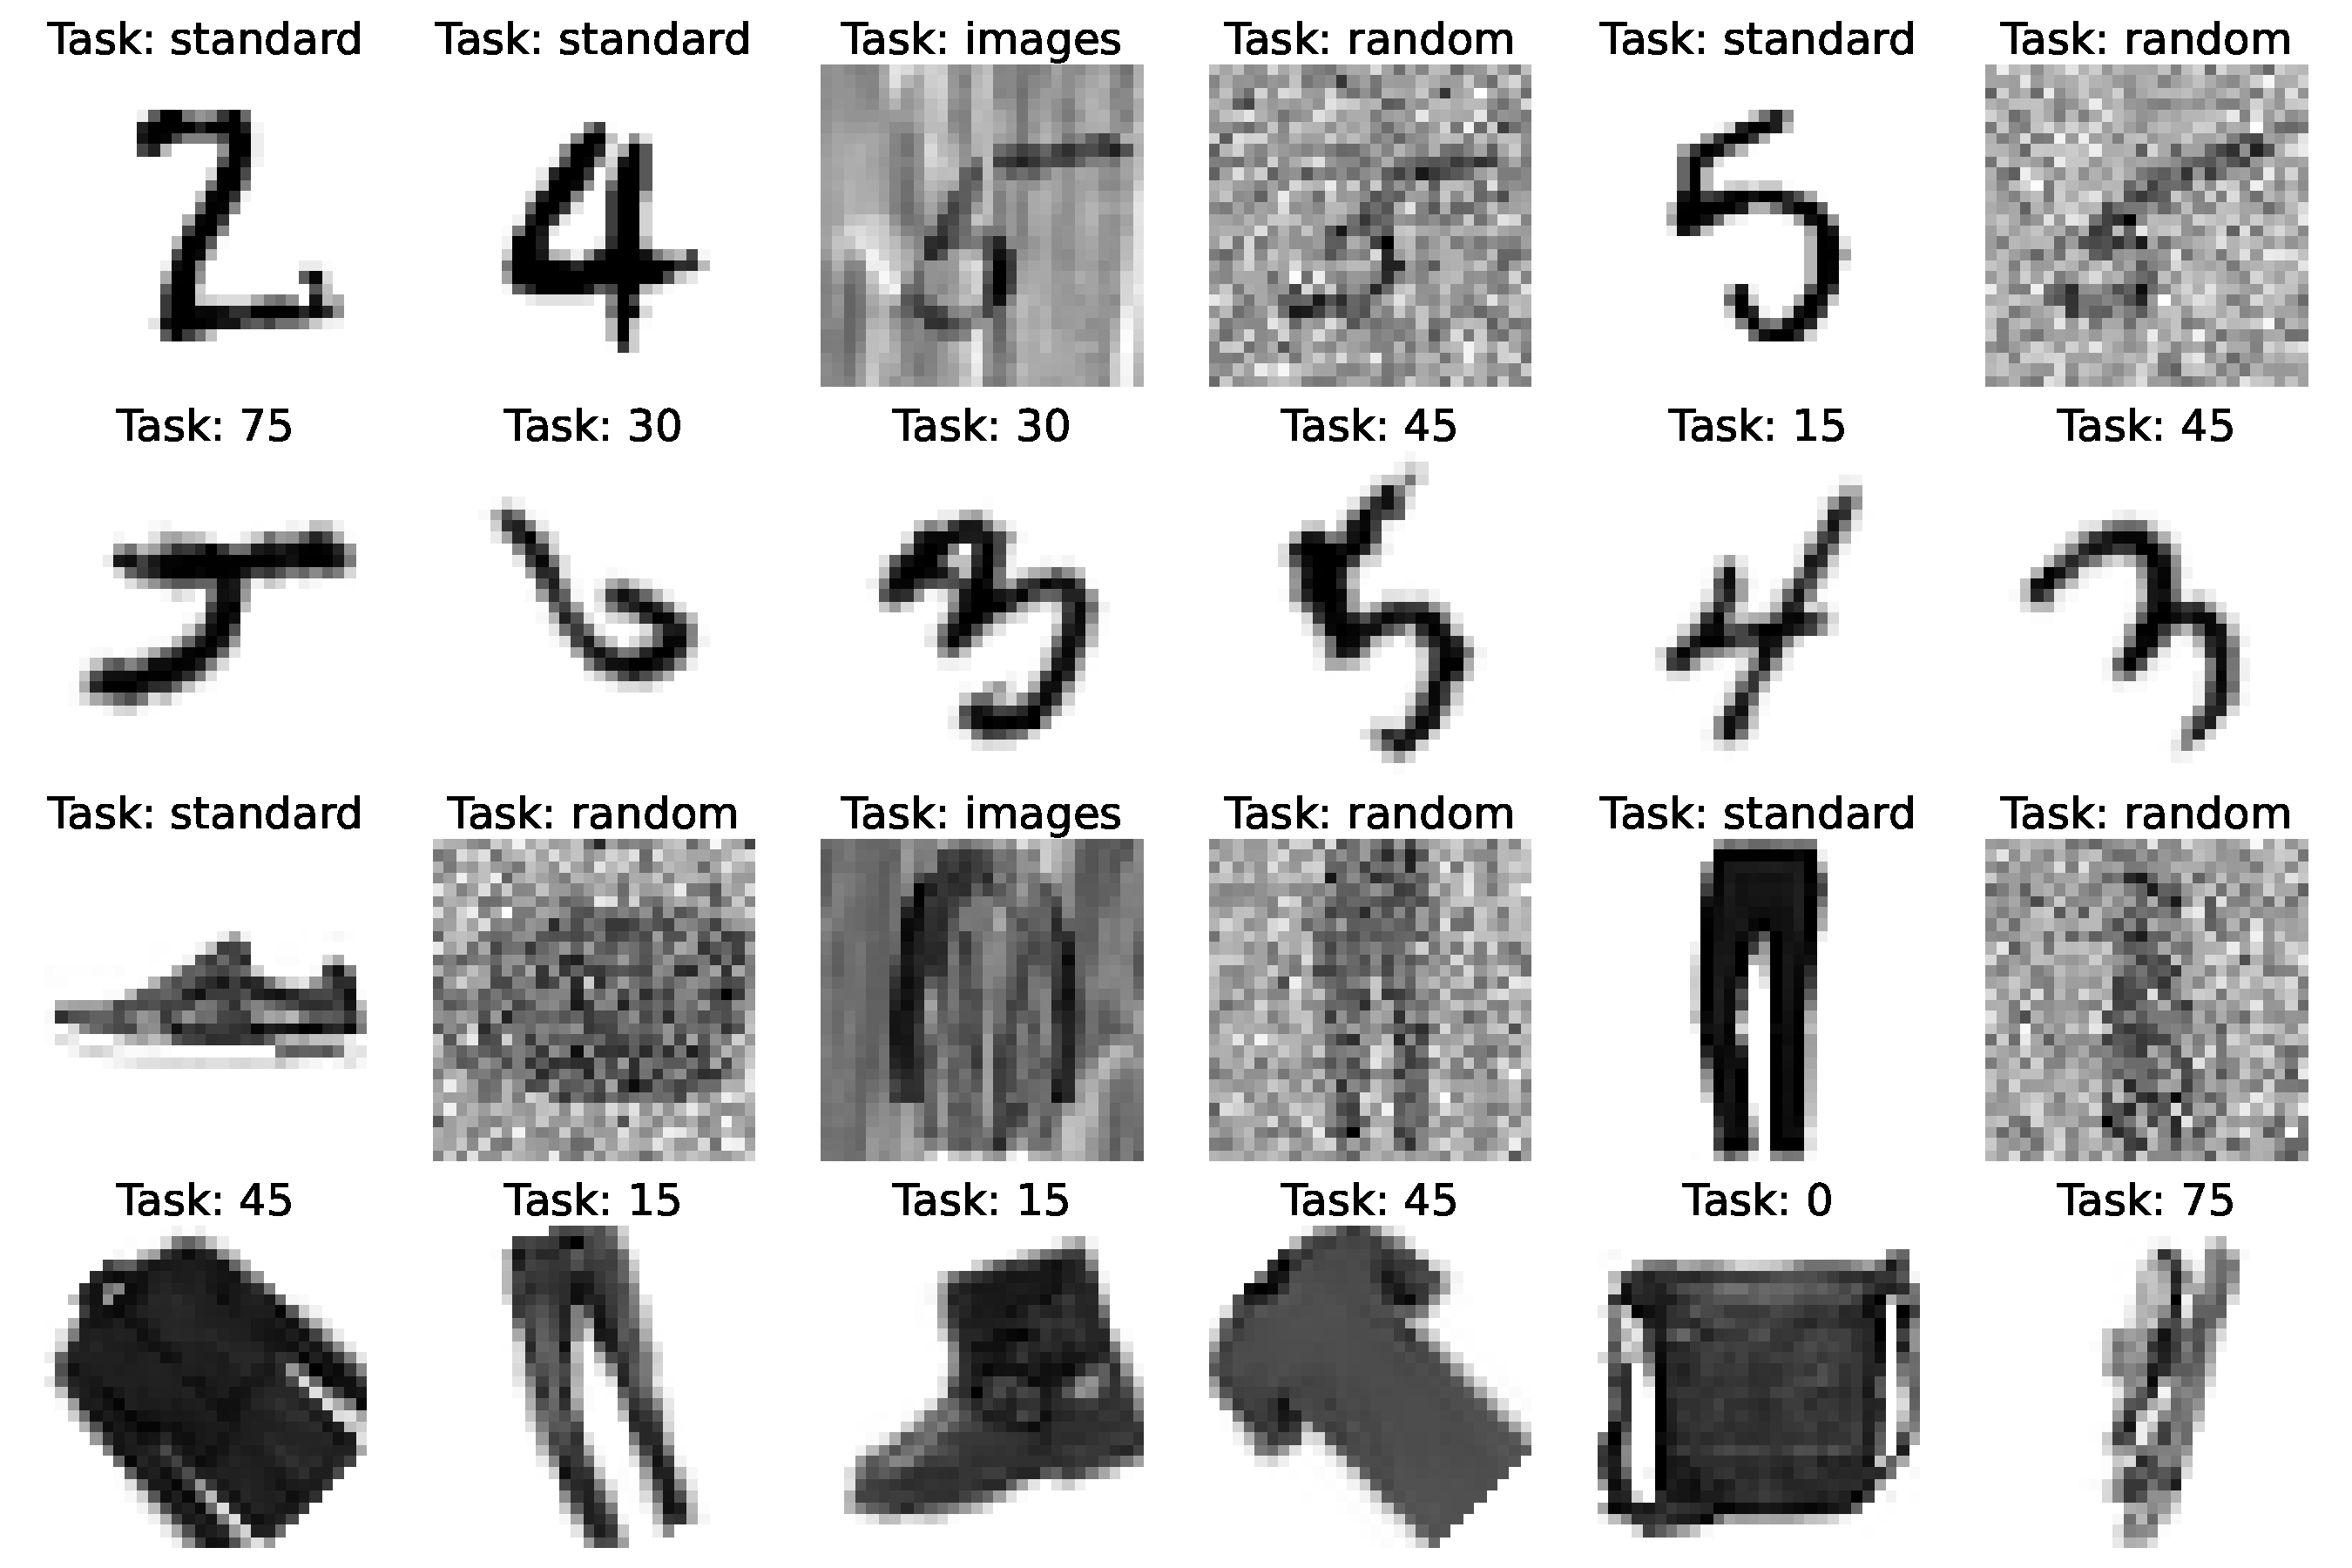
\includegraphics[width=\linewidth]{Chapter4/HAIS2022/hais22_datasets.pdf}
    \caption{Images of the four classification problems used. Each image has a title indicating the corresponding task. The rows correspond to \fdata{var-MNIST}, \fdata{rot-MNIST}, \fdata{var-FMNIST} and \fdata{rot-FMNIST} (from top to bottom).}
    \label{fig:problems_hais2022}
\end{figure}

\paragraph*{Problem Description\\}
To test the convex \acrshort{mtl} neural networks we use four \acrshort{mt} image datasets:
\fdata{var-MNIST}, \fdata{rot-MNIST}, based on MNIST~\citep{LeCunBBH98}, and \fdata{var-FMNIST}, \fdata{rot-FMNIST}, based on fashion-MNIST~\citep{xiao2017}.
%
The MNIST and fashion-MNIST datasets are both composed of \num{70000} examples of $28\times 28$ grey-scale images. The MNIST dataset contains images of handwritten numbers, while the fashion-MNIST has images of clothes and fashion-related objects.
Both are used as classification problems, where the images have to be classified in one of $10$ possible classes, $10$ different digits or $10$ different types of clothes. These classes are balanced in both datasets.
%
To generate the Multi-Task image datasets that we use, we take the images from MNIST or fashion-MNIST and use either the \emph{variations} procedure or the \emph{rotation} one.
%
For the \fdata{var-MNIST} and \fdata{var-FMNIST} we use the \emph{variations} procedure. Inspired by the work of~\cite{BergstraB12}, we consider three transformations:
\begin{itemize}
    \item \textit{random}: adding random noise to the original image.
    \item \textit{image}: adding a random patch of another image to the original image.
    \item \textit{standard}: no transformations are applied to the original image.
\end{itemize}
Then, we use a random split to divide the original datasets in three groups. To each group we apply one of the transformations defined, so we get three tasks: two with \num{23333} examples and the third one with \num{23334}.

%
For the \fdata{rot-MNIST} and \fdata{rot-FMNIST} we use the \emph{rotations} procedure. Using the definitions of~\cite{GhifaryKZB15}, we consider six transformations:
\begin{itemize}
    \item \textit{0}: rotating $0^{\circ}$ the original image.
    \item \textit{15}: rotating $15^{\circ}$ the original image.
    \item \textit{30}: rotating $30^{\circ}$ the original image.
    \item \textit{45}: rotating $45^{\circ}$ the original image.
    \item \textit{60}: rotating $60^{\circ}$ the original image.
    \item \textit{75}: rotating $75^{\circ}$ the original image.
\end{itemize}
Again, we use a random split to divide the original datasets in six groups and each group is applied one of the transformations defined above, so we get six tasks: four with \num{11667} examples and two with \num{11666}.
%

In Figure~\ref{fig:problems_hais2022} we show examples of the four \acrshort{mtl} image problems that we generate, with the corresponding task annotation for each one.



\paragraph*{Experimental Procedure.\\}
% Models Considered
For testing the performance of our proposal we consider the following models:
\begin{itemize}
    \item \fmod{ctlNN}: a \acrshort{ctl}-based neural network, that is, a single network for all tasks.
    \item \fmod{itlNN}: an \acrshort{itl}-based neural network, that is, an independent network for each task.
    \item \fmod{hsNN}: an \acrshort{mtl}-based neural network using the hard sharing strategy. That is, a single neural network is used for all tasks, where the first layers are shared among tasks, but a task-specific output layer is used for each task.
    \item \fmod{cvxmtlNN}: an \acrshort{mtl}-based neural network using the convex formulation we propose.
\end{itemize}
% convNet
All of these models are based on a convolutional network, which we will name \fmod{convNet}, whose architecture is taken from the Spatial Transformer Network~\citep{Jaderberg_2015} implementation given in Pytorch\footnote{\href{www.pytorch.org/tutorials/intermediate/spatial\_transformer\_tutorial.html}{www.pytorch.org/tutorials/intermediate/spatial\_transformer\_tutorial.html}}.
The architecture of \fmod{convNet} consists, in this order, on two convolutional layers of kernel size $5$, with $10$ and $20$ output channels each; then a dropout layer, followed by a max pooling layer, and two fully connected hidden layers with $320$ and $50$ neurons. After this, the output layers follow.

%
Since we use one-hot encoding for the multiple classes, the architecture of the \fmod{ctlNN} consists on a single network with the \fmod{convNet} architecture with $10$ output neurons, one for each class.
%
In the \fmod{itlNN}, an independent network, with the \fmod{convNet} architecture and $10$ output neurons, is used for each task.
%
For the \fmod{hsNN}, a single network with the \fmod{convNet} architecture is used, but we have a group of $10$ output neurons for each task in the problem. For example, if we are using the \emph{rotation}-based problems, we would have $60$ output neurons, but only the group of $10$ corresponding to each task is used with each example.
%
In the \fmod{cvxmtlNN} we use a network with the \fmod{convNet} architecture and $10$ output neurons to model the common network and each of the task-specific networks. That is, given an example from task $r$, the $10$ common output neurons and the  $r$-th task-specific ones are combined to obtain the final output. 

% Optimizer and Hyperparameters
We use the AdamW algorithm~\citep{LoshchilovH19} to train all the models considered, and the weight decay parameter $\mu$ for each model is selected using a CV-based search over the values $\set{10^{-4}, 10^{-3}, 10^{-2}, 10^{-1}, 10^{0}}$. The rest of the parameters, which are part of the architecture, are fixed and set to the default values: the dropout rate is $0.5$ and we use a $2\times 2$ max pooling layer with a stride of $2$.
%
The \fmod{cvxmtlNN} model also has $\lambda$ as a hyperparameter, and it is selected, alongside $\mu$, using a CV grid search, where the grid for $\lambda$ is $\set{0, 0.2, 0.4, 0.6, 0.8, 1}$.

%
The train and test sets are generated using a task-stratified split of $70\%$ and $30\%$, respectively.
The CV grid searches are carried out using the training set, where we use a $5$-fold CV scheme. These folds are task-stratified, that is, all have the same task proportions. Also, since the problems are class-balanced and the sample size is reasonably large, the folds are expected to be class-balanced as well.

\paragraph*{Results.\\}

\begin{table}[t!]
    \centering
        \caption{Test accuracy with majority voting.}
        \label{tab:test_accuracy_majority}
    \begin{tabular}{l*{4}{c}}
        \hline
                           &   \fdata{var-MNIST} &   \fdata{rot-MNIST} &   \fdata{var-FMNIST} &   \fdata{rot-FMNIST} \\
        \hline
         \fmod{ctlNN} &              0.964 &           0.973 &                     0.784 &                  0.834 \\
         \fmod{itlNN} &              0.968 &           0.981 &                     0.795 &                  0.873 \\
         \fmod{hsNN}  &              0.971 &           0.980  &                    0.770  &                 0.852 \\
         \multirow{2}*{\fmod{cvxmtlNN}} &              \fmaxn{0.974} &           \fmaxn{0.984} &                     \fmaxn{0.812} &                  \fmaxn{0.880} \\
         & ($\lambda^* = {0.6}$)  & ($\lambda^* = {0.8}$) & ($\lambda^* = {0.6}$)  & ($\lambda^* = {0.6}$) \\
         \hline
        \end{tabular}
        
\end{table}

\begin{table}[t!]
    \centering
        \caption{Test mean categorical cross entropy.}
        \label{tab:test_crossentropy_mean}
    \begin{tabular}{l*{4}{c}}
        \hline
                           & \fdata{var-MNIST}   & \fdata{rot-MNIST}     & \fdata{var-FMNIST}   & \fdata{rot-FMNIST}   \\
        \hline
         \fmod{ctlNN} & 1.274 $\pm$ 0.143  & 1.145 $\pm$ 0.039 & 2.369 $\pm$ 0.183         & 1.757 $\pm$ 0.075      \\
         \fmod{itlNN} & 1.072 $\pm$ 0.029  & 0.873 $\pm$ 0.058 & 2.356 $\pm$ 0.130         & 1.598 $\pm$ 0.042      \\
         \fmod{hsNN}  & 1.087 $\pm$ 0.253  & 0.898 $\pm$ 0.073 & 3.067 $\pm$ 0.888         & 1.888 $\pm$ 0.075      \\
         \multirow{2}*{\fmod{cvxmtlNN}} & \fmaxn{0.924} $\pm$ \fmaxn{0.024}  & \fmaxn{0.831} $\pm$ \fmaxn{0.029} & \fmaxn{2.147} $\pm$ \fmaxn{0.090}         & \fmaxn{1.482} $\pm$ \fmaxn{0.063}      \\
         & ($\lambda^* = {0.6}$)  & ($\lambda^* = {0.8}$) & ($\lambda^* = {0.6}$)  & ($\lambda^* = {0.6}$)      \\
         \hline
        \end{tabular}
\end{table}

% Refitting models
To get more accurate results, less sensitive to randomness, we train each model $5$ different times. To do this, once the optimal hyperparameters have been selected using the CV in the training set, we refit the model with these hyperparameters using the entire training set. That is, \acrshort{cv} is done only once for each model in each problem, but then we repeat $5$ times the procedure of training the network over the whole training set.

% Accuracy vs Categorical CE
Although maximizing the accuracy is ultimately the goal in classification problems, it is not a differentiable measure, so we use the categorical cross entropy instead as the loss function to train the networks. Both measures are broadly correlated, but they do not represent exactly the same behavior. We will show the results using both for completeness.

% Tables
Since we have $5$ instances of each model, a typical strategy to combine their predictions is majority voting. We perform this majority voting using the logits, in the output neurons, of each instance and averaging them, so we have $10$ values, one for each class.
In Table~\ref{tab:test_accuracy_majority} we show the test accuracy, using the logits average already described, for each of the approaches considered.
%
Other approach to visualize these results is to compute the categorical cross entropy directly on the averaged logits, which we show in Table~\ref{tab:test_crossentropy_mean}.
%
In both tables we also show the optimal values for $\lambda$ selected in the CV.

% Analysis
Our proposal, the \fmod{cvxmtlNN} model, obtains the best results in all the problems, either in terms of accuracy or cross entropy.
The \acrshort{itl} approach comes second in all problems, except for the accuracy score in \fdata{var-MNIST}, where the \fdata{hsNN} is second and \fdata{itlNN} goes third.
The \fdata{hsNN} model goes third in the rest of problems, while the \fdata{ctlNN} gets the worst results consistently in all problems, sometimes by a large margin.
%
By looking at the tables, it seems that a \acrshort{ctl} approach is not able to capture the different properties of each task simultaneously. On the other hand, the \fmod{\acrshort{itl}} approach obtains good results, because it is specialized in each task.
Looking at the optimal values for $\lambda$, there is, however, common information shared among the tasks. These values fall far from the $0, 1$ margins, so neither the \acrshort{ctl} nor the \acrshort{itl} are optimal approaches. This is reflected in the Tables~\ref{tab:test_accuracy_majority} and~\ref{tab:test_crossentropy_mean}, where the \fmod{cvxMTLNN} outperforms consistently \fmod{ctlNN} and \fmod{itlNN}. We can assume, then, that the information learned by the common network and the task-specific ones is complementary, because their combination leads to better results.
%
The hard sharing approach, although better than a \acrshort{ctl} one, seems to be too rigid to effectively capture the differences among different tasks, so it is frequently surpassed by the \acrshort{itl} network.




% Complementing common and task-specific






















\section{Adaptive Graph Laplacian for Multi-Task Learning}





















\section{Conclusions} \label{seq-conclusions}

